%%%%%%%%%%%%%%%%%%%%%%%%%%%%%%%%%%%%%%%%%%%%%%%%%
\documentclass[a4paper,11pt]{article}
\pdfoutput=1 % if your are submitting a pdflatex (i.e. if you have
             % images in pdf, png or jpg format)
\usepackage[top=0.83in,right=1.6cm,left=1.6cm]{geometry}
%\usepackage[a4paper, total={6in, 8in}]{geometry}

\usepackage{jheppub} % for details on the use of the package, please
                     % see the JCAP-author-manual
%\usepackage[english]{babel}
\usepackage{tabu}

%\usepackage{epsfig,epstopdf}  
%\usepackage{graphicx}
%\usepackage{slashed}             
%\usepackage{url}
\usepackage{xcolor}
\usepackage{multirow}
%\usepackage{multicol}

\usepackage{enumitem}
\usepackage{placeins}
%\usepackage{xspace}
%\usepackage{appendix}
\usepackage{hepnames}
%\usepackage{HEPparticles}
\usepackage{comment} 
\usepackage{tocloft}
\usepackage{ptdr-definitions}
\usepackage{rotating}
%\usepackage{subcaption}
%\usepackage{hyperref}
%\usepackage{cite}

\clubpenalty=1000
\widowpenalty=10000
\allowdisplaybreaks
%\setlength\textwidth{6.2in}
%\setmargin\left{.6in}
\newgeometry{width=16.5cm, left=2.2cm, top=2.5cm, bottom=3.5cm}
\setlength{\bibsep}{0cm}
\bibpunct{[}{]}{,}{n}{}{,}

\newcommand{\Wprime}{\PWpr\xspace}

\newcommand{\Pb}{{{\Pqb}}\xspace}
\newcommand{\Pt}{{{\Pqt}}\xspace}
\newcommand{\Ps}{{{\Pqs}}\xspace}
\newcommand{\Pc}{{{\Pqc}}\xspace}
\newcommand{\Pd}{{{\Pqd}}\xspace}
\newcommand{\Pu}{{{\Pqu}}\xspace}
\newcommand{\PAb}{{{{\Paqb}}}\xspace}
\newcommand{\PAt}{{{{\Paqt}}}\xspace}
\newcommand{\PAs}{{{{\Paqs}}}\xspace}
\newcommand{\PAc}{{{{\Paqc}}}\xspace}
\newcommand{\PAd}{{{{\Paqd}}}\xspace}
\newcommand{\PAu}{{{{\Paqu}}}\xspace}

%\renewcommand{\Pl}{\ensuremath{\cmsSymbolFace{l}}\xspace}

%\renewcommand{\PV}{{\ensuremath{{V}}}\xspace}
\renewcommand{\PV}{{{{V}}}\xspace}
%\providecommand{\PV}{{V}\Xspace} % generic vector boson
\newcommand{\VH}{{{\PV}{\PH}}\xspace}

%\renewcommand{\Pl}{\textrm{\Pl}}

\newcommand{\pb} {\mbox{\ensuremath{\,\text{pb}}}\xspace}


%%%%%%%%%%%%%%%%%%%%%%%% Abstract %%%%%%%%%%%%%%%%%%%%%%%%%%


\begin{document}
\title{A SM-EFT analysis of Higgs-strahlung processes}

\author[a]{Suman Chatterjee,}
\emailAdd{suman.chatterjee@oeaw.ac.at}

\affiliation[a]{Institute of High Energy Physics of the Austrian Academy of Sciences (HEPHY)}

%\maketitle

\section*{Project description}

\tableofcontents

\newpage

%------------------------------------------------
\section{Science}\label{sec:sciience}

Since the start of operations in 2008, the Large Hadron Collider (LHC) at CERN has provided a data set amounting to about $10^{16}$ proton-proton collisions that are expected to double, once more, until 2024.
During the LHC Run~2 (2015--2018), the CMS experiment~\cite{CMS_ex} collected  $137\fbinv$ of proton-proton collision data at $\sqrt{s}=13\TeV$ and is now performing extensive analyses to extract the maximum knowledge on fundamental particle physics processes at the \TeV scale.
The most prominent key milestone in the LHC experiments' history is the discovery of the Higgs boson~(\PH), jointly announced by the ATLAS and CMS Collaborations in 2012~\cite{Aad:2012tfa,Chatrchyan:2012ufa}.
It completed the particle content of the standard model (SM) of particle physics. 
Since then, precision measurements of the Higgs boson's mass~\cite{CMS:2017dib,CMS:2020xrn}, its charge-parity (CP) nature~\cite{CMS:2019jdw,CMS:2020cga}, its couplings to electroweak gauge bosons ($\PW^{\pm}$, \PZ,~\Pgg), and other couplings have been at the center of the LHC research program with many already entering the precision regime.
% not needed->?
%third-generation fermions (\Pb, \Pt), $and second-generation leptons (\Pmu)~\cite{CMS-PAS-HIG-19-005}, among others.
\begin{comment}
\begin{itemize}
\item Discovery of Higgs boson (\PH) in 2012~\cite{Aad:2012tfa,Chatrchyan:2012ufa} resulting in the completion of the standard model (SM) of particle physics. 
This is followed by precision measurements of Higgs boson properties, such as mass~\cite{CMS:2017dib,CMS:2020xrn}, CP nature~\cite{CMS:2019jdw,CMS:2020cga}, coupling to gauge bosons, third-generation fermions, and second-generation leptons~\cite{CMS-PAS-HIG-19-005}, among others.
\item Precision measurements of processes involving electroweak gauge bosons (\PW, \PZ, \Pgg), light- and heavy-flavor quarks (\Pu, \Pd, \Ps, \Pc, \Pb, \Pt), gluons (\Pg).
\item Discovery of processes not observed previously in colliders, such as light-by-light scattering~\cite{CMS:2018erd}, single-production of a top quark in association with a \PZ boson~\cite{CMS:2018sgc}, vector boson scattering~\cite{CMS:2017fhs}, among others.
\item Constraining a large region of parameter space in models beyond the SM (BSM) constructed with extended symmetries 
constructed to explain several observed phenomena and to provide an explanation of theoretical quests.
\end{itemize}
\end{comment}
At the same time, the lack of smoking-gun evidence for resonant phenomena beyond the SM~(BSM) has restricted many sophisticated models, like supersymmetry or models with extra dimensions, that were conceived to cure the SM's shortcomings: 
the absence of a suitable dark matter candidate, the unknown origin of nonzero neutrino masses, the baryon asymmetry of the universe, and the lack of a theoretical explanation of the fine tuning required for the insensitivity of the Higgs boson mass to quantum corrections. 
%Supersymmetry, a viable model of dark matter candidate or models with extra dimensions have not been discovered. 

Is the case, therefore, closed? 
In this proposal, I argue on the contrary. 
In fact, the recent application of effective field theories~(EFT)~\cite{Grinstein:1991cd,Chiu:2007dg,Passarino:2016pzb} demonstrates impressively that subtle deviations, hiding in the observables' distributions, can probe BSM phenomena at energy scales often exceeding the LHC's reach in the direct searches. 
The underlying theoretical framework considered in this proposal is the SM effective field theory~(SM-EFT)~\cite{Jenkins:2013zja,Alonso:2013hga,Jenkins:2013wua,Englert:2014cva,Brivio:2017vri} that systematically extends the SM with operators of higher mass dimension that smoothly change the kinematic spectra.
Specifically,  SM-EFT modifications to the SM Higgs sector result in deviations that grow with the momenta of the final state particles. 
The joint production of a \PH boson and a vector boson (\VH with \PV$=\PW^{\pm},\PZ$) are particularly strongly affected, turning the highly energetic \VH final states into extremely important discovery tools for BSM phenomena. 
In addition to the changes in one-dimensional kinematic distributions, 
BSM sources of CP violation change subtle triple-correlations of angular observables that are easily lost if not targeted explicitly by means of ``interference resurrection''~\cite{Panico:2017frx}.
The latter techniques have been demonstrated in the simpler $\PW\gamma$ final states~\cite{CMS-PAS-SMP-20-005}, but the order-of-magnitude sensitivity gain for precision measurements, although proposed recently~\cite{Banerjee:2019twi}, has not yet been exploited experimentally in the Higgs sector. 
% FIXME Instead of the following, make a nice list of UV models you actually constrain and list them in Section 5. --> Done (added in Sec. 4)
% For example, the existence of a heavy gauge boson of mass beyond the LHC reach can manifest itself modifying {\PH}-{\PV} couplings~\cite{Appelquist:1974tg}. 
% The second most dominant mechanism of Higgs boson production at LHC is in association with a vector boson, referred to as \VH production, which involves a $s$--channel vector boson. 

To close these gaps, I propose an extensive measurement of the \PH--\PV couplings in \VH final states. 
Resurrecting the process' interference pattern and simultaneously leveraging the signature of energy growth in the kinematic tails of the \PH, $\PW^{\pm}$, and \PZ bosons promise unique sensitivity and a wide reach to SM-EFT effects, including the CP structure of the coupling.
The proposed analysis includes differential cross section measurements of a number of observables never considered before.
Combining \PH boson decays to a pair of \Pb quarks with the requirement of leptonic \PV decays~(electrons or muons) leads to a high signal acceptance while suppressing the complex hadronic backgrounds.  

% FIXME -> Methodology? --> Done (first sentence of Sec. 5.1)
%The \VH production with \PV decaying to leptons is an ideal place to probe \PH in its dominant decay mode to a pair of \Pb quarks as the leptons can be used to select the targeted events at the trigger-level and also to reduce the multijet background from quantum chromodynamics (QCD) interaction.

% FIXME -> Research hypothesis (or maybe drop) --> Dropped
%The production of \PV from quark-antiquark annihilation, the associated production of \PH from \PV, and the decay of \PH to a pair of \Pb quarks are sensitive to the footprint of new physics at respective vertices, namely vector couplings, gauge couplings, and Yukawa couplings. %in $\PH \to \Pb \PAb$ decay. 
% FIXME -> I added the following information in the research hypothesis. --> Thanks!
%A number of such couplings involving the Higgs boson can be directly probed for the first time at LHC~\cite{Gupta:2014rxa}. The rest of the couplings, which could have left signatures in earlier experiments like LEP, can also be probed with better accuracy at LHC because of the increase of their impact with energy~\cite{Ellis:2014jta,Grojean:2018dqj}.

% FIXME -> Can drop, already used above.  --> Dropped
%The \VH production also gives an unique opportunity to probe the CP-sensitivity in \PH--\PV coupling,  which can be probed using novel techniques developed very recently, known as interference resurrection~\cite{Panico:2017frx}, not explored so far in the Higgs sector. The proposal changes the scenario in the area of experimental measurements.  

%The work can start with the data set already collected during the LHC's Run~2. 
Sensitivity to the SM-EFT effects mentioned previously can already be obtained using the existing data set collected during the LHC Run~2. 
With the additional $160\fbinv$ of data to be delivered by the LHC during Run~3 (2022--2024), these measurements are expected to have a significant leap in precision. 
In the remainder of the proposal, I attempt to demonstrate these claims.



\section{Research hypothesis}
\label{sec:research_hypo}

%\subsection{Effective field theory couplings in \PV($\to$ \Pl\Pl)\PH($\to$ \Pb \PAb) production}

I assume that there exist no unknown resonances within the kinematic reach of LHC and 
the {\TeV}-scale phenomena are described by the standard model effective theory (SM-EFT). 
The SM-EFT progressively includes operators of mass dimension greater than four that respect the SM symmetries~\cite{Jenkins:2013zja,Alonso:2013hga,Jenkins:2013wua,Englert:2014cva,Brivio:2017vri} and is defined by the Lagrangian
\begin{equation}
\mathcal{L}_{\text{SM-EFT}} = \mathcal{L}_{\text{SM}} +  {\sum}_{i} \frac{\text{c}_i^{\left(5\right)}}{\Lambda} \mathcal{O}_{5,i} + {\sum}_{i} \frac{\text{c}_i^{\left(6\right)}}{{\Lambda}^{2}} \mathcal{O}_{6,i} + ... \;.
\label{Eq:SMEFT}
\end{equation}
It captures all non-resonant BSM phenomena below an arbitrarily chosen energy scale $\Lambda$.
The dimensionless Wilson coefficients $\text{c}^{\left(n\right)}$ are used to parameterize the effects on observables, while the terms $\mathcal{O}_5$ and $\mathcal{O}_6$ are  the operators at mass dimensions 5 and 6, respectively.
The only possible dimension-5 candidate is the  Weinberg operator~\cite{PhysRevLett.43.1566}, not relevant for the phenomenology of this proposal ~\cite{Bonnet:2009ej}.
% FIXME -> let's not discuss what we don't want to discuss.
%the smallness of neutrino mass points to the relevance of this operator only at energy much higher than that relevant for LHC physics. 
% FIXME -> Too much, I think ... (hermiticity, 2010)
%The complete set of non-redundant operators at  dimension-6, except for the Hermitian conjugates, written for the first time in 2010 forms the so-called Warsaw basis~\cite{Grzadkowski:2010es}. 
The number of baryon and lepton number conserving dimension-6 operators is 2499 when all flavor degrees of freedom are counted. There are 76 operators respecting a $\textrm{U}(3)^5$ flavor symmetry~\cite{Alonso:2013hga} among which the 12 listed in Table~\ref{Tab:Operators} affect the \VH process.
The operators are written in the so-called Warsaw basis~\cite{Grzadkowski:2010es}, and it is the central aim of this proposal to constrain their Wilson coefficients via their effects on the Higgs boson production properties and decay kinematics~\cite{Hagiwara:1993qt,Ellis:2014dva,Murphy:2017omb,Baglio:2020oqu}.

\begin{table}[tph]
\caption{
The dimension-6 operators in the Warsaw basis~\cite{Grzadkowski:2010es} affecting \VH  processes at leading order.
}
\begin{center}
{\renewcommand{\arraystretch}{1.3}
\begin{tabular}{lcl|lcl}
${\cal O}^{(1)}_{Hq}$&&$i H^\dagger \overleftrightarrow{D}_\mu H \bar{q}   \gamma^\mu q$&${\cal O}_{HWB}$&&$ H^\dagger \sigma^a H W^a_{\mu\nu}B^{\mu\nu}$ \\
\rule{0pt}{4ex} ${\cal O}^{(3)}_{Hq}$&&$i H^\dagger \sigma^a \overleftrightarrow{D}_\mu H \bar{q}  \sigma^a \gamma^\mu q$ &${\cal O}_{H\tilde{W}B}$&&$ H^\dagger \sigma^a H W^a_{\mu\nu}\tilde{B}^{\mu\nu}$\\
\rule{0pt}{4ex} ${\cal O}_{Hu}$&&$i H^\dagger \overleftrightarrow{D}_\mu H \bar{u}_R  \gamma^\mu u_R$&${\cal O}_{H{W}}$&&$(H^\dagger H)\,W_{\mu\nu}{W}^{\mu\nu}$\\
\rule{0pt}{4ex} ${\cal O}_{Hd}$&&$i H^\dagger \overleftrightarrow{D}_\mu H \bar{d}_R  \gamma^\mu d_R$&${\cal O}_{H\tilde{W}}$&&$ (H^\dagger H)\, W^a_{\mu\nu}\tilde{W}^{a \mu\nu}$\\
\rule{0pt}{4ex} ${\cal O}_{HD}$&&$(H^\dagger  {D}_\mu H)^*(H^\dagger  {D}_\mu H)$& ${\cal O}_{HB}$&&$(H^\dagger H)\,B_{\mu\nu}B^{\mu\nu}$\\
\rule{0pt}{4ex} ${\cal O}_{H\square}$&&$(H^\dagger H) \square (H^\dagger H)$& ${\cal O}_{H\tilde{B}}$&&$(H^\dagger H)\,B_{\mu\nu}\tilde{B}^{\mu\nu}$
%\hline
\end{tabular}}
\label{Tab:Operators}
\end{center}
\end{table}

The operators ${\cal O}^{(1)}_{Hq}$, ${\cal O}^{(3)}_{Hq}$, ${\cal O}_{Hu}$, and ${\cal O}_{Hd}$ introduce the 4-point interactions depicted in Fig.~\ref{fig:Feynman_digarams} (left). 
Together with ${\cal O}_{HD}$ and ${\cal O}_{HWB}$, these six operators describe all relevant \PV-fermion coupling modifications (Fig.~\ref{fig:Feynman_digarams}, middle). 
The remaining operators modify the \PH--\PV coupling, shown in Fig.~\ref{fig:Feynman_digarams} (right). 
There is also the Yukawa-type operator $H^\dagger H \bar{Q}H b$, which only changes the $\PH \to \Pb \PAb$ branching ratio and, thus, can be probed in an inclusive cross section measurement. 
\begin{figure*}[hbtp]
\begin{center}
%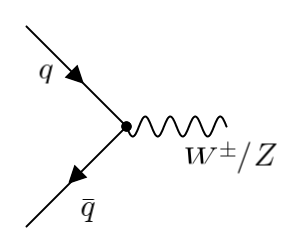
\includegraphics[width=0.3\textwidth]{Figures/Feynman_diagrams/Vff.png}
%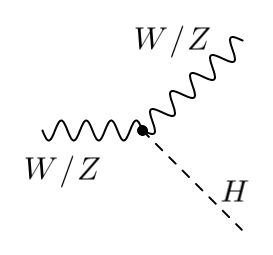
\includegraphics[width=0.3\textwidth]{Figures/Feynman_diagrams/hVV.png}
%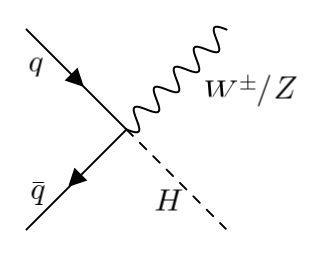
\includegraphics[width=0.3\textwidth]{Figures/Feynman_diagrams/ffVh.png}
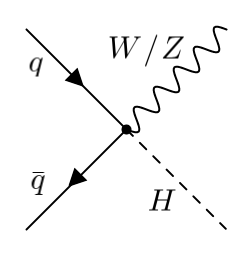
\includegraphics[width=0.3\textwidth]{Figures/New/LHE//qqVH.png}
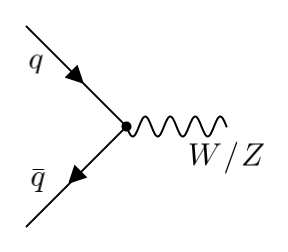
\includegraphics[width=0.3\textwidth]{Figures/New/LHE//qqV.png}
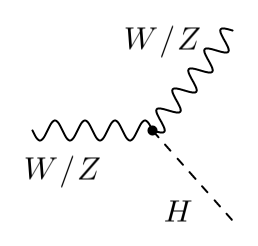
\includegraphics[width=0.3\textwidth]{Figures/New/LHE//VVh.png}
\end{center}
\caption{
Feynman diagrams for \VH production sensitive to different dimension-6 operators.
%The energy growth induced by the diagrams in \VH production cross section are the following: $E^0$ (left), $E$ (middle), $E^2$ (right). 
}
\label{fig:Feynman_digarams}
\end{figure*}

%\subsection{Direct measurements of SM-EFT couplings in \PV($\to \Pl \Pl $) \PH ($\to \Pb \PAb$)}

%SM-EFT parameters can, in general, be constrained using data from the previous low-energy experiments by replacing \PH by its vacuum expectation value ($v$) in operators in Table~\ref{Tab:Operators}. For a majority of the operators at work here, which are of the form ${\PH}^2\mathcal{L}_{\text{SM}}$,
%this just corresponds to a shift of the parameters in SM Lagrangian. 
%Therefore, those can be probed directly for the first time at LHC.

The $\textrm{SU}(2)$ doublet \PH is expanded as $\begin{pmatrix} 0 \\ v+h \end{pmatrix}$, where $v$ is the vacuum expectation value  and $h$ corresponds to the physical Higgs boson.
At the weak scale,  \PH is replaced by $v$ in operators shown in Table~\ref{Tab:Operators}, and some of them can be constrained using the existing collider results from  the LEP and the Tevatron experiments.
Nevertheless, the bounds from the LHC are expected to be more stringent~\cite{Ellis:2014jta,Grojean:2018dqj}.
Moreover, the operators of the form ${\PH}^2\mathcal{L}_{\text{SM}}$, can be directly probed for the first time at the LHC~\cite{Gupta:2014rxa}. 

The energy dependence of the \VH production cross section is critical for the sensitivity of the proposed analyses. 
The Feynman diagram with four-point interaction (Fig.~\ref{fig:Feynman_digarams}, left) involves one scalar and one vector field and two fermion fields.
%thus, the corresponding operator expansion has the form $\frac{v}{{\Lambda}^2} E^5$ in high energy limit.
%Therefore, the exponent in $S$-matrix, $\int L d^{4}x$, takes the form  $\sim \frac{vE}{{\Lambda}^2}$, 
Power counting with naive dimensional analysis~\cite{Manohar:1983md} implies a scaling of the cross section with $E^2$. 
%after replacing \PH by $v$, 
The diagram with the modification of the fermion--\PV coupling (Fig.~\ref{fig:Feynman_digarams}, middle) 
%the diagram in Fig.~\ref{fig:Feynman_digarams} (left)
corresponds to a Lagrangian term  of the form $\frac{v^2}{{\Lambda}^2} V_{\mu} \bar{\psi} {{\gamma}^{\mu}} {\psi}$, which does not induce a cross section enhancement with energy. 
The operators modifying \PH--\PV coupling (Fig.~\ref{fig:Feynman_digarams}, right) give rise to terms $vh {\partial}^{\mu}{\partial}^{\nu} V_{\mu}V_{\nu}$.
%$\sim (\frac{v^2}{2}+vh+\frac{h^2}{2}) ({\partial}^{\mu}{\partial}^{\nu} V_{\mu}V_{\nu} + ...)$, 
%which goes as $\frac{vE}{{\Lambda}^2}$ in high energy limit. 
When interfering with the SM term $(H^{\dagger}H) V^{\mu}V_{\mu}$, this gives rise to a linear increase of cross section with energy.
%FIXME One sentence about power counting and energy growth. Then come the angles below ... --> Done
%FIXME -> Drop? Is the BSM acceptance really relevant anywhere? --> Dropped for now
%The methodology used in conventional measurements of SM-EFT operators assumes that all the object and event selection conditions have the same efficiency and acceptance for the SM and SM-EFT operators, which is known to be not the case always, and also miss important subtle effects by integrating over a number of important variables.% as will be shown in Sec.~\ref{sec:method}.
The proposed measurement will probe the operators in Table~\ref{Tab:Operators} 
using kinematic variables exhibiting energy growth and, for the first time, the angular structure that is sensitive to subtle interference effects.
At high energy, the \PH boson has large \pt, and its decay products are collimated in a single large-radius jet, thus providing a testbed for the application of the cutting-edge jet substructure techniques~\cite{Qu:2019gqs,Sirunyan:2020lcu}.
For the angular information, we exploit the techniques of Ref.~\cite{Banerjee:2019twi} and define the angles and decay planes of the \VH process as shown in Fig.~\ref{fig:HelicityFrame}.
% FIXME Here please describe concretely the angular amplitudes. Eq. 3.6 from Spannowsky, mention how these integrated to zero, and note the CP structure. --> Done 

% not only allow to disentangle energy growth induced by different operators, but also provide an unique opportunity to sense the additional sources of CP violation due to dimension-6 operators in SM-EFT.
\begin{figure*}[hbtp]
\begin{center}
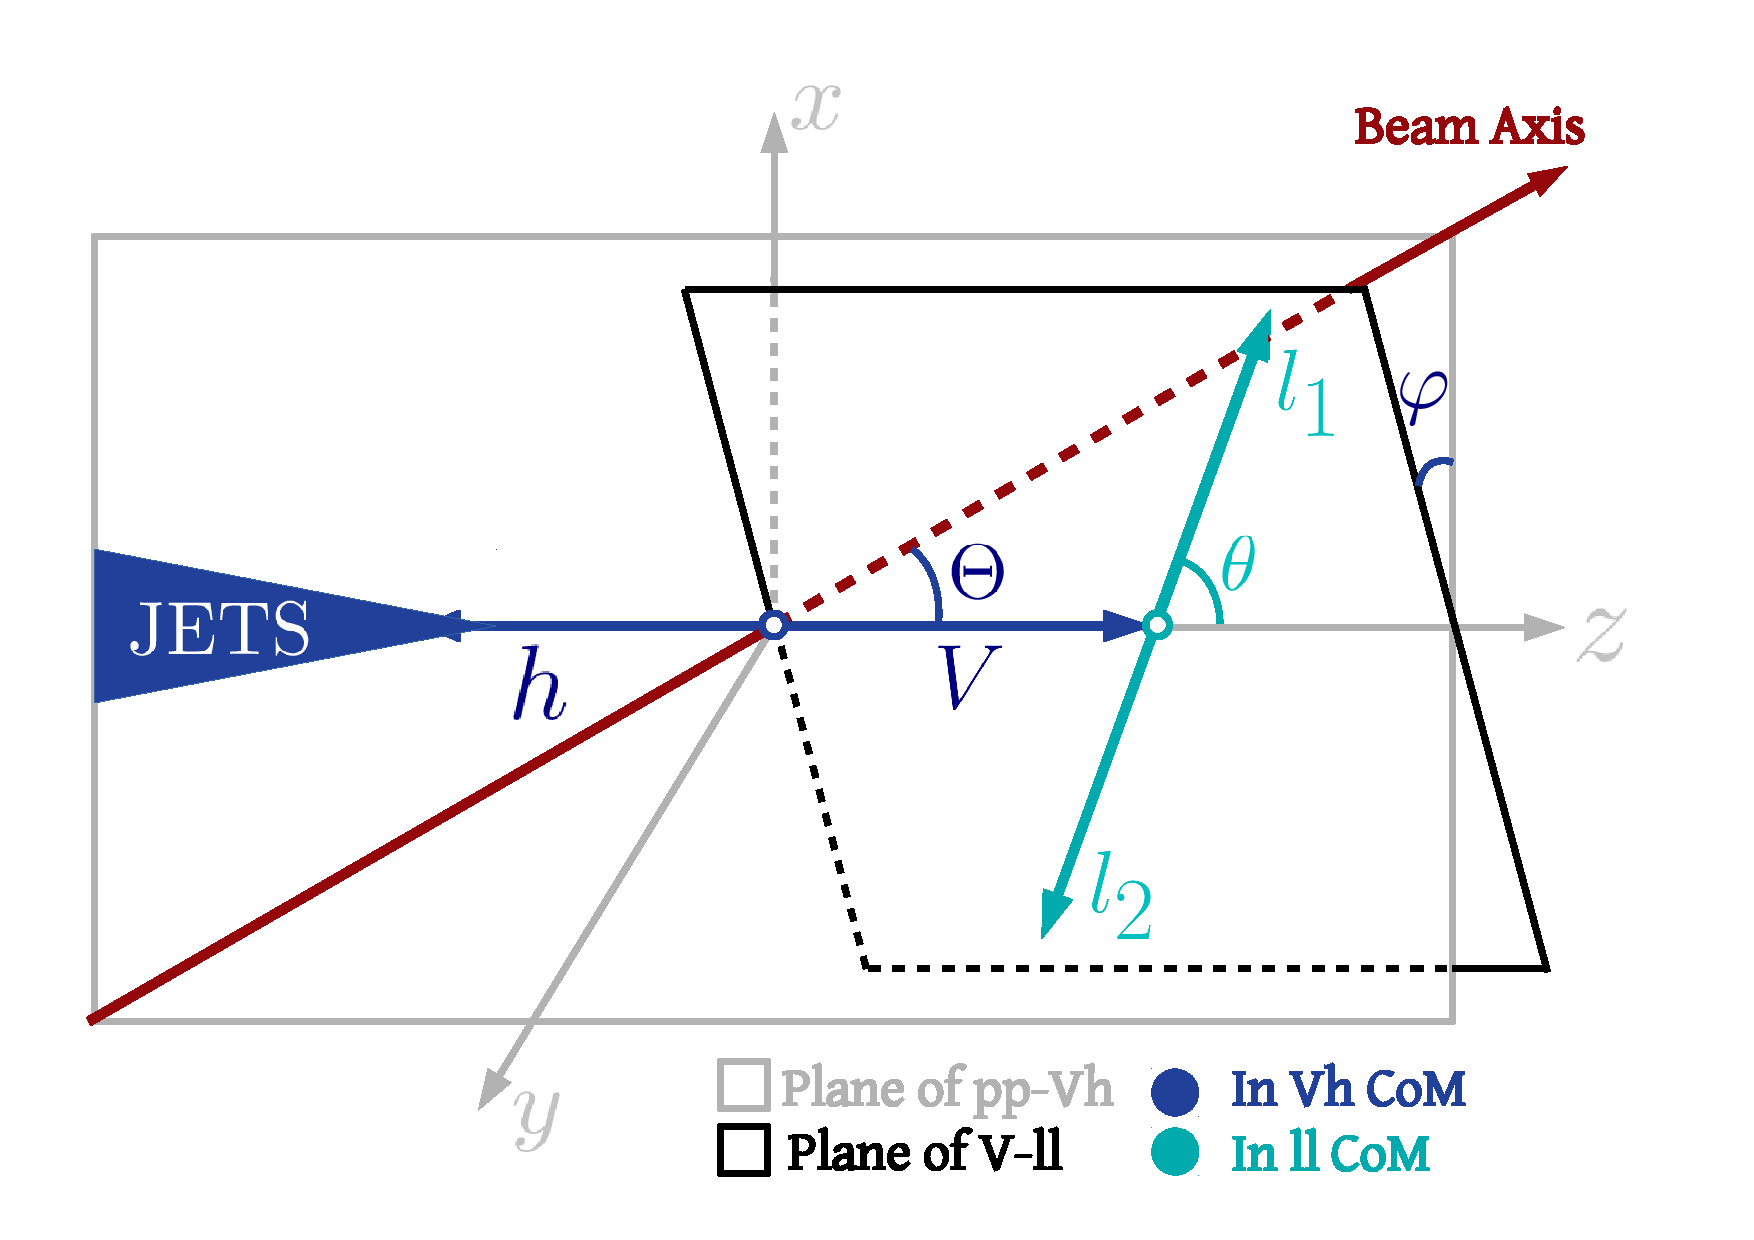
\includegraphics[width=0.75\textwidth]{Figures/LHE/TheThreeAnglesVh.pdf}
\end{center}
\caption{
Decay planes and angles in the \PV($\rightarrow \textrm{\Pl} \textrm{\Pl}$)\PH($\rightarrow \Pb \PAb$) production. Note that $\Theta$ is defined in the $\textrm{\PV}\PH$ rest frame, while $\theta$ is defined in the \PV rest frame.
}
\label{fig:HelicityFrame}
\end{figure*}

The squared amplitude of \PV($\to \Pl \Pl$)\PH($\to \Pb \PAb$) production, when summing over the lepton helicities, has the form
\begin{equation}
	|\mathcal{M} \left(\hat{s}, \Theta, \theta, \varphi \right)|^{2} = {\sum}_{i} a_i \left(\hat{s}\right) f_i \left(\Theta, \theta, \varphi \right),
\label{Eq:Amplitude}
\end{equation}
where $a_i\left(\hat{s}\right)$ are functions of Wilson coefficients and the energy transfer $\hat{s}$ involved in the process.
The functions $f_i$ depend on the three angles in Fig.~\ref{fig:HelicityFrame}

{\renewcommand{\arraystretch}{1.3}
\begin{table}[h!]
\begin{tabular}{lcl}
    $f_{1} = f_{LL} = \sin^{2}\Theta \sin^{2}\theta$, && $f_{6} = \tilde{f}^{\,1}_{LT} = \sin\varphi \sin\Theta \sin\theta, $\\
    $f_{2} = f^1_{TT} = \cos\Theta \cos\theta$, &&$f_{7} = \tilde{f}^{\,2}_{LT} = \sin\varphi \sin\Theta \sin\theta \cos\Theta \cos\theta$,\\
    $f_{3} = f^2_{TT} = (1+\cos^{2}\Theta)(1+ \cos^{2}\theta)$, && $f_{8} = f_{TT'} = \cos^{2}\varphi \sin^{2}{\Theta} \sin^{2}{\theta}$,\\
    $f_{4} = f^1_{LT} = \cos\varphi \sin\Theta \sin\theta$,&& $f_{9} = \tilde{f}_{TT'} =  \sin^{2}{\varphi} \sin^{2}{\Theta} \sin^{2}{\theta}$,\\
    $f_{5} = f^2_{LT} = \cos\varphi \sin\Theta \sin\theta \cos\Theta \cos\theta$
    %\label{Eq:funcs}
\end{tabular}
\end{table}
}
\vspace{-1.4cm}\begin{equation}
\phantom{x}\label{Eq:funcs}\end{equation}
\noindent where indices refer to the polarizations of the intermediate vector boson.


A traditional inclusive measurement implicitly integrates over $\Theta, \theta, \varphi$, thus removing all the terms in Eq.~\eqref{Eq:funcs}, except $f_{LL}$ and $f^2_{TT}$. 
This is the cause of loss of important information, which can be recovered for $f^2_{LT}$, $\tilde f^{\,2}_{LT}$, $f_{TT'}$, and $\tilde f_{TT'}$  by using a triple differential analysis with respect to all three angles. 
Because the incoming quark and anti-quark direction is not known at the LHC, the terms proportional to $f^1_{TT}$, $f^1_{LT}$, and $\tilde{f}^1_{LT}$ can not be extracted.

\begin{comment}
Now, the operators at Table~\ref{Tab:Operators} can also be constrained using the existing measurements in Higgs sector at LHC~\cite{CMS-PAS-HIG-19-005,ATLAS:2020fcp,ATLAS:2020jwz}. 
However, this methodology assumes that all the object and event selection conditions have the same efficiency and acceptance for the SM and SM-EFT operators, 
which is known to be not the case always. 
Also, as will be shown in Sec.~\ref{sec:method}, some important effects can be lost in traditional measurements of kinematic variables. 
Therefore, it is necessary to construct a set of observables that can extract telltale signatures of EFT operators without any loss of information. 
Also, the impact of all the conditions applied at the analysis level needs to be checked for the operators involved. 
These goals can only be achieved in a dedicated measurement as proposed here.
\end{comment}


\section{Objectives}
\label{sec:objective}

\begin{figure*}[t]
\begin{center}
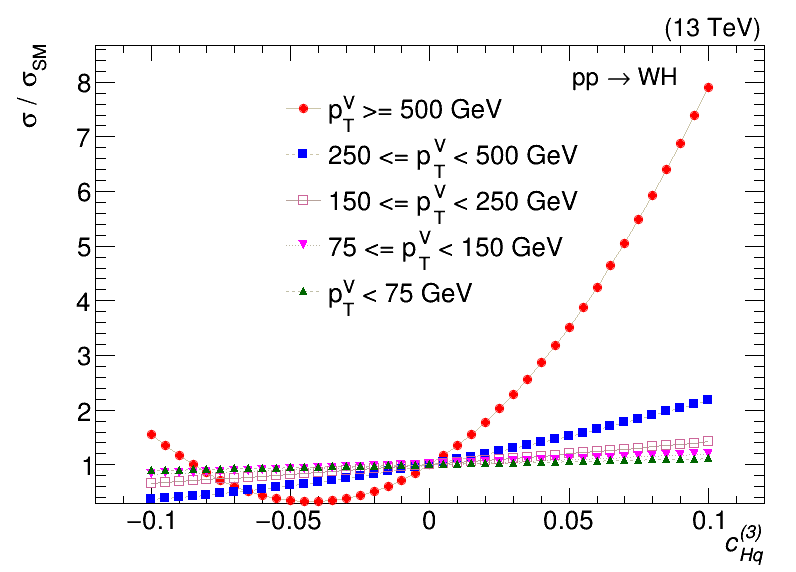
\includegraphics[width=0.321\textwidth]{Figures/New/LHE/WH/Canv_cpq3i.png}
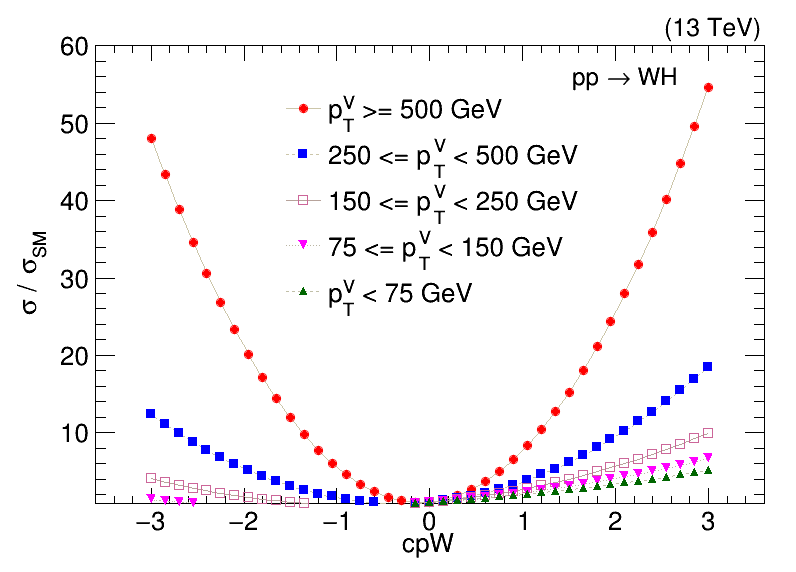
\includegraphics[width=0.321\textwidth]{Figures/New/LHE/WH/Canv_cpW.png}
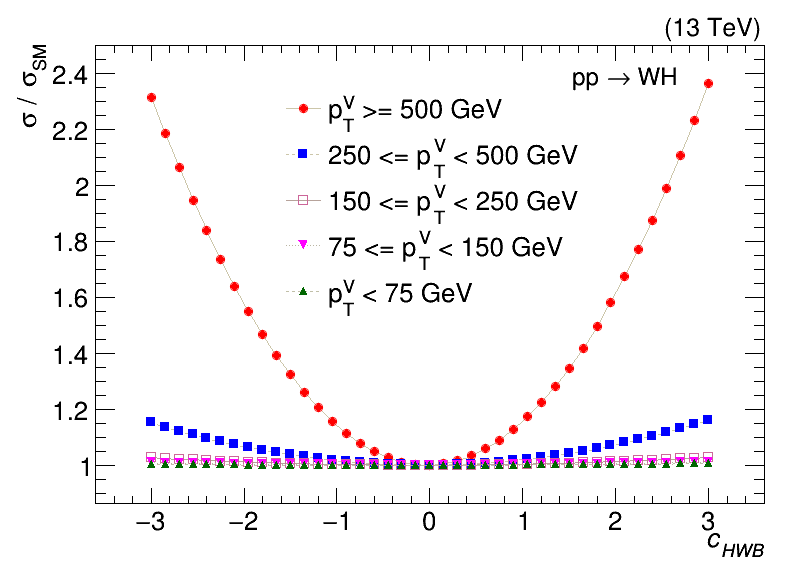
\includegraphics[width=0.321\textwidth]{Figures/New/LHE/WH/Canv_cpWB.png}
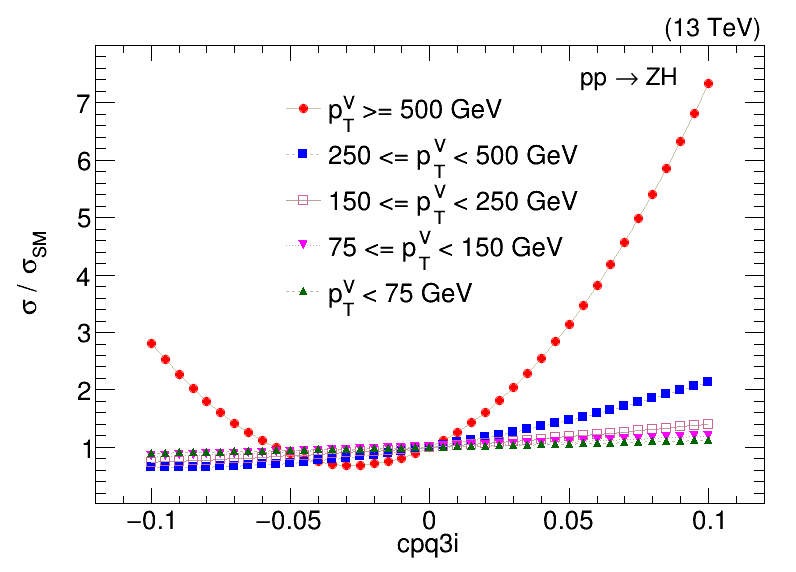
\includegraphics[width=0.321\textwidth]{Figures/New/LHE/ZH/Canv_cpq3i.png}
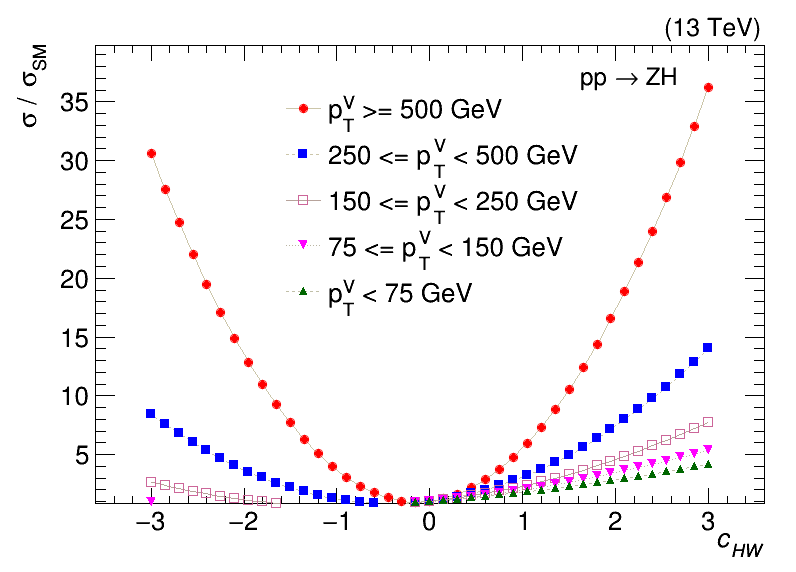
\includegraphics[width=0.321\textwidth]{Figures/New/LHE/ZH/Canv_cpW.png}
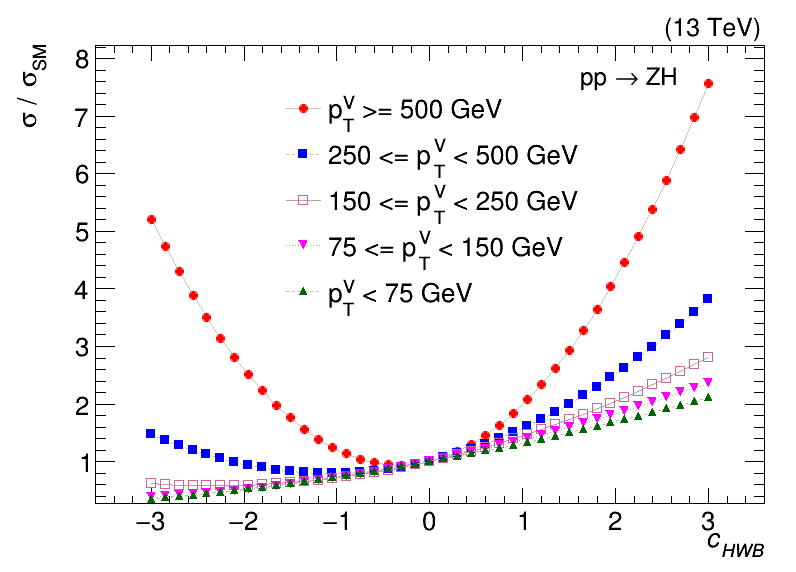
\includegraphics[width=0.321\textwidth]{Figures/New/LHE/ZH/Canv_cpWB.png}
\end{center}
\caption{
The ratio of the cross section of the $\PW\PH$ (top) and $\PZ\PH$ (bottom) processes relative to the SM prediction, $\sigma/\sigma_{\textrm{SM}}$, as a function of Wilson coefficients corresponding to operators ${\cal O}^{(3)}_{Hq}$ (left), ${\cal O}_{HW}$ (middle), and ${\cal O}_{HWB}$ (right), respectively, in five regions of $\PW$ and $\PZ$ boson {\pt}.
}
\label{fig:LHE_WZH}
\end{figure*}
The goal of the proposal is to probe the SM-EFT operators in Table~\ref{Tab:Operators} as precisely as possible using events from the \VH processes in the data collected by the CMS experiment during the LHC Run 2 and 3. 
Two experimental objectives separately tackle the energy dependence of the differential cross section and the CP nature of \PH--\PV coupling due to SM-EFT effects.
At the final stage of the work, those will be combined to achieve optimal sensitivity.

%In the first objective, I will exploit energy growth 
The first objective is the exploitation of energy growth
induced by SM-EFT operators
%4-point SM-EFT interactions 
to boost the sensitivity of differential cross section measurements in \VH production with leptonic \PV decays.
Latest jet substructure techniques for boosted \PH bosons will be applied for this purpose.
The three operators ${\cal O}^{(3)}_{Hq}$, ${\cal O}_{HW}$, ${\cal O}_{HWB}$, their CP-odd counterparts, and the operators ${\cal O}_{HD}$, ${\cal O}_{H\square}$ affect both $\PW\PH$ and $\PZ\PH$ productions. 
The dependence of the production cross section on the first three Wilson coefficients for different selections in vector boson transverse momentum, $\pt(\PV)$ is shown in Fig.~\ref{fig:LHE_WZH}. 
The energy growth is visible as an increased dependence on the Wilson coefficient for selections with higher $\pt(\PV)$. %FIXME <- Tell them what they see! --> Done
The operators ${\cal O}^{(1)}_{Hq}$, ${\cal O}_{Hu}$, ${\cal O}_{Hd}$, ${\cal O}_{HB}$, and ${\cal O}_{H\tilde{B}}$ affect only the $\PZ\PH$ production, 
because both left- and right-handed initial-state quarks of same flavor take part in $\PZ\PH$ production, while only the left-handed quarks of different flavors are involved in $\PW\PH$ production~\cite{Falkowski:2014tna,Banerjee:2018bio}. 
Therefore, simultaneous measurements of the couplings in both the $\PW\PH$ and the $\PZ\PH$ processes are necessary to confidently probe the complete set of relevant operators~\cite{Banerjee:2019twi}.
%Therefore, measurements in both $\PW\PH$ and $\PZ\PH$ production are essential to probe the complete set of dimension-6 operators affecting $\PV\PH$ production.
%FIXME Can this be made more concrete? What helicity structure is responsible? --> Done
%Also, a reference is needed. --> Done
%What is the purpose of this statement? --> The answer is now given in the last sentence of the last part of this section mentioning this point
The SM cross section for $\PW\PH$ production with  $\PH\rightarrow\Pb\PAb$ and $\PW\rightarrow\ell\nu$  is 0.28\pb, whereas it is only 0.06\pb for $\PZ\PH$ production, where $\PZ\rightarrow\ell\ell$.
Thus, the $\PW\PH$ process provides better statistical precision in the measurements. 
%FIXME Quote the x-sec numbers! --> Done
The \PZ final state is less populated, 
but contributions from background processes are smaller, 
particularly at high energy, 
providing an independent sample to measure the sensitivity to SM-EFT operators and 
two processes together can lead to evidence of the BSM signal if any of the Wilson coefficients are found to be significantly different from zero.
%corroborating evidence of the BSM signal.
%As mentioned previously, $\PZ\PH$ production is affected by a number of operators which do not participate in $\PW\PH$ production. % because of the helicity structure of incoming quarks.


%In the second objective, I use the
The second objective is the use of
angular observables to further boost the sensitivity and tackle the CP-structure of the \PH--\PV interaction. 
As an example, 
distribution of one of the angular variables, $\varphi$, is shown in Fig.~\ref{fig:LHE_phi}. 
Here, the leading contribution for the CP-even and -odd operators come from the terms corresponding to $f^{2}_{LT}$ and $\tilde{f}^2_{LT}$ in Eq.~\eqref{Eq:funcs}, respectively, which have $\cos\varphi$ and $\sin\varphi$ dependence.
%FIXME <- Here a link to the sinusodial variations is needed from Sec. 3. It should be stated that sin/cos is CP odd/even. Let's add a sentence when the table is there. --> Done
In the simpler $\PW\gamma$ final state, the technique increased the sensitivity to interference between the SM and the SM-EFT operator of interest by about a factor of 10~\cite{CMS-PAS-SMP-20-005}.
Section~\ref{sec:method} presents a preliminary sensitivity study for the three most important operators. 
%In the final work, the optimum set of operators will be chosen using the Fisher information matrix.
%The experimental work to excavate two distinct features, combined to achieve optimal sensitivity, are tackled separately.

\begin{figure*}[tph]
\begin{center}
%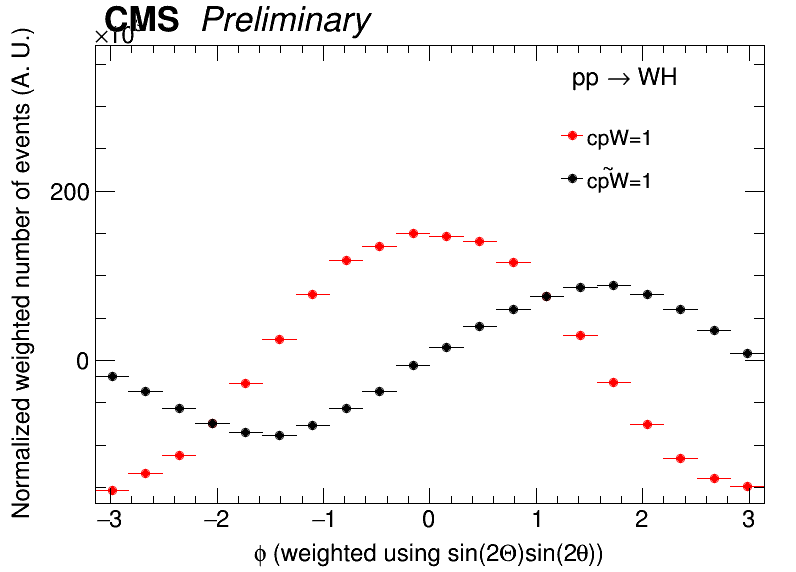
\includegraphics[width=0.45\textwidth]{Figures/LHE/WH/LHE_Plot_phi.png}
%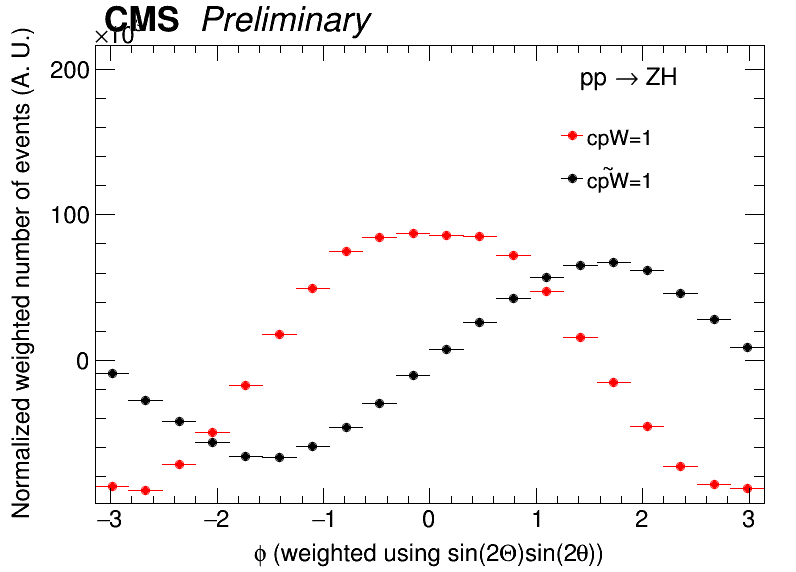
\includegraphics[width=0.45\textwidth]{Figures/LHE/ZH/LHE_Plot_phi.png}
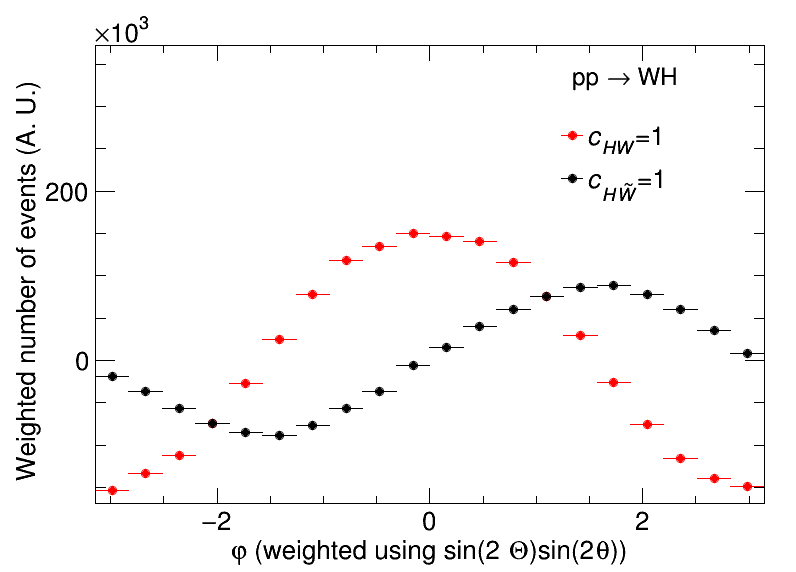
\includegraphics[width=0.45\textwidth]{Figures/New/LHE/LHE_Plot_phi_WH.png}
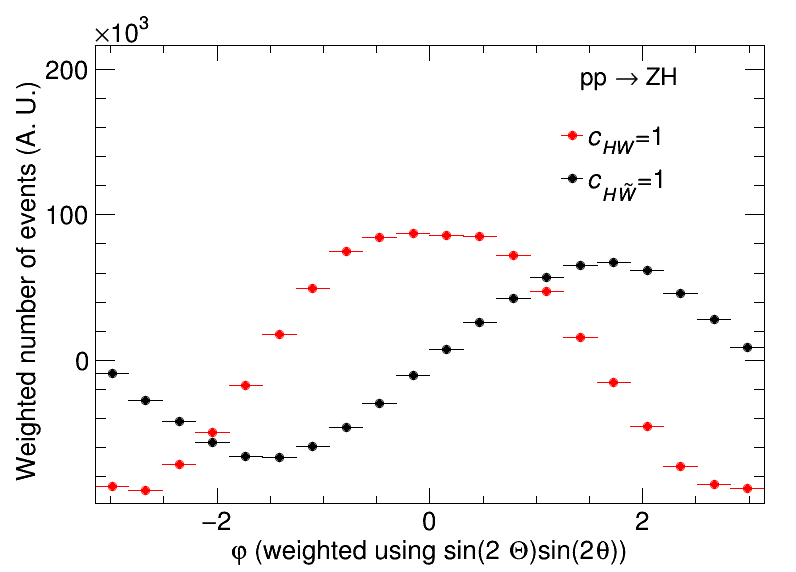
\includegraphics[width=0.45\textwidth]{Figures/New/LHE/LHE_Plot_phi_ZH.png}
\end{center}
\caption{
Distribution of angle $\varphi$ at the particle level for Wilson coefficients corresponding to CP-even operator ${\cal O}_{HW}$  (red points) and CP-odd operator ${\cal O}_{H\tilde{W}}$ (black points) set to 1 in case of $\PW\PH$ (left) and $\PZ\PH$ (right) productions.
For each entry in the distribution, a weight of $+1$ or $-1$ is applied depending on the sign of $\sin\left(2\Theta\right) \sin\left(2\theta\right)$. 
}
\label{fig:LHE_phi}
\end{figure*}



\section{Scientific originality}

%Although the SM-EFT operators can be indirectly probed using results from the previous experiments, 
%The combined data sets from the LHC Run 2 and the future LHC Run 3 provide an opportunity to measure SM-EFT operators involving the Higgs field~\cite{Elias-Miro:2013mua,Gupta:2014rxa} with unprecedented precision. 
In the $\textrm{\PV}\rightarrow\Pl\Pl$ and $\PH\rightarrow\Pb\PAb$ final state, I extend traditional search strategies, based on the simplified template cross section binning scheme~\cite{Berger:2019wnu}, by angular observables sensitive to subtle SM-EFT effects and the CP-structure of the \PH--\PV interaction. For the first time,

%So far, there exist very few measurements where all the efficiency and acceptance effects of object and event selection conditions are taken into account, and complete information contained in an event is used.
%The proposed measurement will extend the scope of probing new physics scenarios in the following ways.

\begin{itemize}

\item the complete multi-dimensional event information is used in \VH production to directly probe dimension-6 SM-EFT operators inducing energy growth.
Besides kinematic event properties, novel angular variables~(Fig.~\ref{fig:angles}) crucially refine the analysis strategy. 
They disentangle the various SM-EFT effects and can largely boost the sensitivity~\cite{CMS-PAS-SMP-20-005}. Furthermore, %  up to an order of magnitude~\cite{CMS-PAS-SMP-20-005}. Furthermore, 

\item the angular information, not explored previously in \VH production, is used to probe the CP structure of SM-EFT modifications of the \PH--\PV coupling. We can, therefore, measure new sources of CP violation beyond the SM.
\end{itemize}

A recent differential cross section measurement with an EFT interpretation of the Run~2 data set by the ATLAS collaboration~\cite{ATLAS-CONF-2021-051} includes measurement regions with boosted \PH candidates but ignores the angular information. The most recent EFT interpretation of \VH measurement is restricted to inclusive measurements
\cite{CMS-PAS-HIG-19-005}. The scope of this proposal significantly extends beyond both cases.

Smaller novel items of this proposal pertain to the multivariate analysis~(MVA) strategy employed to achieve these goals. 
%In the journey to achieve the goals, there will be possibilities to improve the techniques used in experimental measurements. 
For example, the proposer's group has recently developed a new technique to train tree-based classifiers to optimally separate effects of SM-EFT operators from the SM background~\cite{Chatterjee:2021nms}.
%Development of the methods and applying those in a CMS measurement by the same group will greatly accelerate the preparation of the results. 
%Also, efficiency of the deep neural network (DNN) based algorithms, used to identify \PH decaying to a pair of \Pb quarks, is conventionally measured in data and simulation in $\Pg \to \Pb \PAb$ process. 
%However, \Pg and \PH are very different in mass, spin, and color properties. During the proposed work, an effort will be pursued to improve the calibration of the tagger, 
%particularly using $\PZ \to \Pb \PAb$ decay.
The combined data sets from the LHC Run~2 and the future LHC Run~3 provide an opportunity to measure SM-EFT operators involving the Higgs field~\cite{Elias-Miro:2013mua,Gupta:2014rxa} with unprecedented precision.

\section{Relevance to the research field}

On a broad scale, the measurements provide a new piece of the {\TeV}-scale SM-EFT puzzle. 
The findings will be interpreted in the context of SM-EFT, which guarantees maximal independence from model assumptions and a smooth interface for theory interpretations.  

The absence of hints for resonant BSM phenomena has shifted the focus from ultraviolet-complete theories to EFTs, with first attempts at complete {\TeV}-scale characterizations emerging relatively recently~\cite{Ellis:2018gqa,Ellis:2020unq,Ethier:2021bye}.
At the experimental collaborations, the measurements of SM-EFT operator coefficients have just arrived at the center stage of the LHC physics program~\cite{CMS:2021nnc,CMS:2021aly,CMS:2021gme}.
The interest from the theoretical and experimental communities is still growing, reflected in various new working groups (e.g., the  LHC EFT working group~\cite{LHC_EFT_WG}) and lecture series (e.g., ``All things EFT''~\cite{All_EFT}).

%The main relevance of the proposed research is to provide a novel building block for the characterization of BSM phenomena at the \TeV energy scale.


In particular, the proposed research contributes a unique probe of SM-EFT operator coefficients in the Higgs sector.
Besides the sensitivity boost from novel experimental techniques, it also complements the existing results by extending to CP-sensitive angular observables, tightly constraining the \PH--\PV couplings.
A deviation from the SM hinting at new sources of CP-violation will have wide-ranging significance in the explanation of the origin of the matter-antimatter asymmetry of the universe~\cite{Cohen:1997ac,Damgaard:2015con,Grzadkowski:2018nbc}.

%In particular, measurements of the vector couplings involving light quarks nicely complement the measurement of the similar couplings involving top quarks and they together can probe the flavor universality in quark sector in SM-EFT.

%Guided by, e.g., the effective description of beta decay in Fermi's theory~\cite{Fermi:1934hr} and Yukawa's theory of meson exchange~\cite{Yukawa:1935xg} EFTs ~\cite{Grinstein:1991cd,Alonso:2013hga,Brivio:2017vri,Passarino:2016pzb}  towards EFT as the future

The relevance of the proposed research extends to adjacent fields when the interplay of LHC measurements in global SM-EFT analysis is considered~\cite{Ellis:2018gqa,Ethier:2021bye}.
For example, specific assumptions of the BSM flavor structure provide a tight connection of the proposed measurement with the sector of top-quark physics. 
Moreover, the SM electroweak symmetry breaking relates the 4-point interactions in Table~\ref{Tab:Operators} to complementary measurements of the fermion-gauge boson couplings. 
An example of this link can be obtained from Fig.~\ref{fig:Feynman_digarams}~(left) when replacing the \PH boson line with $v$.

The results obtained from the proposed measurements can also be reinterpreted as constraints on ultraviolet-complete new physics models describing the underlying dynamics at high energy.
Examples of models the proposed analysis will be capable of probing are the following:
\begin{itemize}

\item Singlet scalar models, where a scalar field, singlet under the SM gauge group, is introduced~\cite{deBlas:2014mba,Profumo:2014opa}. This class of models gives rise to operators of the form of ${\cal O}_{H\square}$, ${\cal O}_{HD}$, ${\cal O}_{HW}$, ${\cal O}_{HB}$, ${\cal O}_{HWB}$, ${\cal O}_{Hu}$, and ${\cal O}_{Hd}$.

\item Models predicting the existence of a new vector boson~\cite{delAguila:2010mx}, for example, \PZprime and \PWprime. 
The models with extra spatial dimensions~\cite{Burdman:2006gy}, and little Higgs models~\cite{PhysRevD.10.275} fall in this category.
If the new bosons coupling to both fermions and gauge bosons have large masses ($>$ few \TeV), they give rise to the contact interaction shown in Fig.~\ref{fig:Feynman_digarams} (left) and thus contributes to the operators  ${\cal O}^{(1)}_{Hq}$, ${\cal O}^{(3)}_{Hq}$, ${\cal O}_{Hu}$, and ${\cal O}_{Hd}$. 

\item Colored extensions of the SM with vector-like quarks (VLQs), triplet under SU(3) and singlet under SU(2)$_L$~\cite{delAguila:2000aa,Dawson:2012di}. 
When VLQs are allowed to couple to light quarks, they can give rise to ${\cal O}^{(1)}_{Hq}$ and ${\cal O}^{(3)}_{Hq}$ operators.
New physics models with \PZprime or VLQs are in highlights in recent times to explain the anomalies in the flavor sector. 

\end{itemize}

The phenomenological implications of the \PH--\PV coupling measurement thus radiate into neighboring research areas, while the proposed experimental program is self-contained.
In the following section, I aim to establish that. 
%Also, an extensive and precise EFT measurement forms a basis that can be used beyond its immediate goals.

\section{Method}
\label{sec:method}

%Achieving goals in time requires setting up a concrete plan in advance. 
We target to use the combined data set collected by the CMS experiment during the LHC Run~2, corresponding to an integrated luminosity of 139\fbinv at $\sqrt{s}=13\TeV$, and the LHC Run~3, currently estimated at $160\fbinv$.
%With $45\%$ of the data available, we can develop and publish novel analysis techniques during the third running period. 
%When the full data set is available at the end of Run~3, we can obtain ultimate precision on a comparably short time scale and publish a benchmark result whose precision can not be surpassed until well into the upcoming high-luminosity LHC research program.
In the following, we report 
%the results of 
a feasibility study of the proposed measurements and exemplify the key methodology.
Important sources of systematic uncertainty modeling the differences of the simulation to data are considered. 
%While the clean $\PZ\PH$ process serves as an independent search channel with orthogonal SM-EFT sensitivity, we focus on the more challenging $\PW\PH$ final states.
We focus on the $\PW\PH$ final states with challenging background rates. The results are also valid for the $\PZ\PH$ process, which provides independent measurement channels with orthogonal SM-EFT sensitivity, higher signal purity, but lower signal yield.
%The results are equally valid for the $\PZ\PH$ case.

\subsection{Final states and observables}

In the SM, the $\PH\rightarrow\Pb \PAb$ decay channel has the largest branching ratio, motivating to choose it for improving  the statistical precision of the measurement.
Leptonic decay modes of the vector bosons help in reducing 
%difficult backgrounds 
the contribution
from multijet production in quantum chromodynamics (QCD).
Therefore, we consider the $\PW\PH$ and $\PZ\PH$ production processes with the $\PW\rightarrow\Pl\Pgn$, $\PZ\rightarrow{\Pl}^{+} {\Pl}^{-}$, and $\PH\rightarrow\Pb\PAb $ decay channels, where $\ell=(\Pe, \Pmu)$.
%=(\Pe, \Pmu)$.

%The following final states are considered.
%\begin{itemize}
%\item $\PW\left(\to \Pl \Pgn \right) \PH \left(\to \Pb \PAb %\right)$
%\item $\PZ\left(\to {\Pl}^{+} {\Pl}^{-} \right) \PH \left(\to \Pb \PAb \right)$
%\end{itemize}


As shown in Sec.~\ref{sec:objective} and Fig.~\ref{fig:LHE_WZH}, the 4-point interactions provided by the operators in Table~\ref{Tab:Operators} induce  energy growth, modifying the high-energy tail of distributions of kinematic observables such as the transverse momenta, $\pt(\PW)$, $\pt(\PZ)$, or $\pt(\PH)$. 
However, these kinematic observables alone are not sufficient to disentangle the various effects from a large number of possible SM-EFT operators. 
A systematic analysis of helicity amplitudes in \VH production followed by vector boson decay is provided in Ref.~\cite{Banerjee:2019twi}. 
Amplitudes involving the longitudinal and transverse vector boson polarizations contribute differently to \VH production in SM and SM-EFT. 
The interference among helicity amplitudes, including CP effects, is preserved at the event level in subtle angular triple-correlations. 
%FIXME Specify when table is there. --> Done
For example, the cosinusoidal and sinusoidal modulations in $\varphi$ distributions shown in Fig.~\ref{fig:LHE_phi} are obtained after using the sign of $\sin\left(2\Theta\right)\sin\left(2\theta\right)$ as seen from $\tilde{f}^2_{LT}$ and $f^2_{LT}$ terms, respectively, in  Eq.~\ref{Eq:funcs}. 
This triple angular correlation allows extracting rich information about the event structure from a joint analysis of kinematic and angular variables.
%
%Specifically, Ref.~\cite{Banerjee:2019twi} proposes to reconstruct the novel angular variables shown in Fig.~\ref{fig:HelicityFrame}. 
It is important to note that traditional strategies can not disentangle the subtle angular triple-correlation: integrating over any of the angles in the final observables removes the interference effects~\cite{Panico:2017frx}.

While SM-EFT effects in background processes, e.g. from diboson production, are ignored for this simple feasibility study, they will be considered in the final measurement.

\begin{comment}
once calculates helicity amplitudes in \VH center-of-mass frame and the cross section has the following form:
\begin{equation}
{\sigma}_{\VH} (\hat{s},\Theta,\theta,\varphi) = {\sum}_{i=1}^{9} a_{i}(\hat{s}) f_{i}(\Theta,\theta,\varphi)	\ .
\label{Eq:Xsection}
 \end{equation}  
In Eq.~\eqref{Eq:Xsection}, $a_{i}$, parameterizing the dependence of Wilson coefficient and energy transfer $\hat{s}$, are known as angular moments and $f_{i}$ encapsulates the dependency on the angles $\Theta,\theta,\varphi$ defined in Fig.~\ref{fig:HelicityFrame}.
\begin{figure*}[hbtp]
\begin{center}
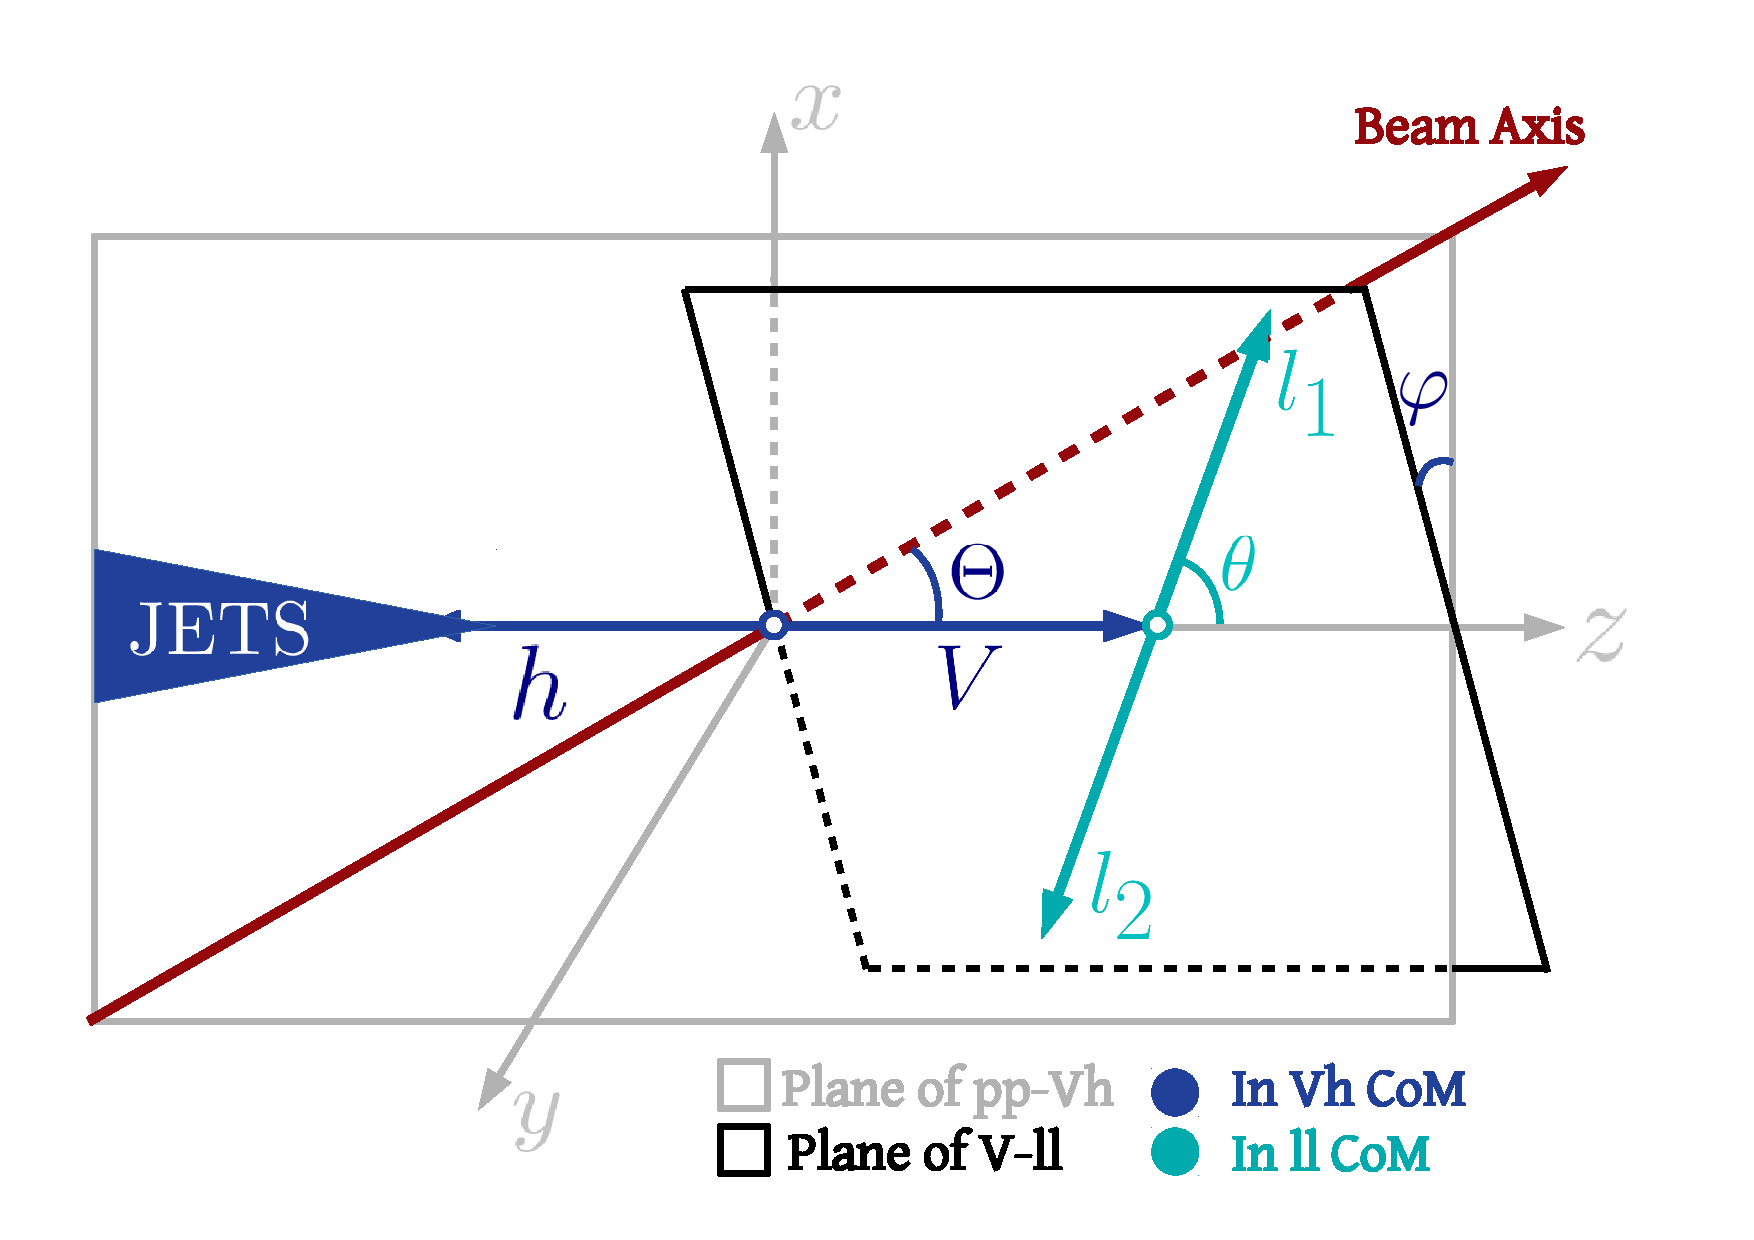
\includegraphics[width=0.75\textwidth]{Figures/LHE/TheThreeAnglesVh.pdf}
\end{center}
\caption{
Definition
}
\label{fig:HelicityFrame}
\end{figure*}
The functions $a$ and $f$ contain the complete information of how \VH production is affected by dimension-6 SM-EFT operators and their forms can be found in Ref.~\cite{Banerjee:2019twi}. 
However, the absence of knowledge about the directions of incoming quark and anti-quark leads to the vanishing of three angular moments. Among the remaining six angular moments, two correspond to the case where the vector boson is either transversely or longitudinally polarized, and the remaining four correspond to the interference of two amplitudes with different polarizations of the vector boson. An inclusive measurement over all the angles leads to the vanishing of the latter four angular moments, thus lossing information about the event structure. 

In this proposal, we target to use complementary kinematic and angular observables in the \VH process and probe the SM-EFT operators at work.


We consider the final states as follows.
\begin{itemize}
\item $\PW\left(\rightarrow \Pl \Pgn \right) \PH \left(\rightarrow \Pb \PAb \right)$
\item $\PZ\left(\rightarrow \Pl \Pl \right) \PH \left(\rightarrow \Pb \PAb \right)$
\end{itemize}
Since $\PH\rightarrow\Pb\PAb$ has the largest branching ratio, its use enables to improve the statistics of the analyzed event sample. 
Leptonic decay of the vector boson helps to get rid of the background from the multijet production in QCD, which is the dominant background in most of the hadronic final states. 
The lepton(s) from the vector boson also helps to trigger the events. The process $\PZ\left(\rightarrow \Pgn \Pgn \right) \PH \left(\rightarrow \Pb \PAb \right)$ is ignored here since we need the lepton directions to construct the angular variables.
\end{comment}

\subsection{Event preselection and categorization}

%The CMS trigger system selects the \VH events based on the presence of leptons~(electrons or muons) originating from the \PW or \PZ bosons. 
%At moderate momenta, single- and double-lepton triggers are used.
%%%The trigger system, developed centrally within the CMS Collaboration, is used to select events with at least one lepton (\Pl) satisfying a threshold in {\pt}.
%At high $\pt\textrm{(\PV)}$, backup trigger paths requiring considerable hadronic activity are used to recover efficiency losses for events with highly asymmetrical \PV decay or with a highly energetic electron. 
%
%The measurement of the trigger selection efficiency ratio between data and simulation is a standard (but important) step towards reducing the total systematic uncertainty.
%For this purpose, we use tag-and-probe methods with $\PZ \rightarrow {\Pl}^{+} {\Pl}^{-}$ events to obtain event-level correction factors that scale the simulation to the data. 
%For the remainder of the feasibility study, we assume that simulation correctly predicts the trigger selection efficiency. 
All results are obtained from events generated with \texttt{Madgraph5\_aMC@NLO}~\cite{Alwall:2014hca} and simulated up to the CMS detector level. 
The SM-EFT effects in the \VH signal are incorporated with \texttt{MadWeight}~\cite{Artoisenet:2008zz} and using the \texttt{SMEFTsim}~model~\cite{Brivio:2017btx}.

The CMS trigger system selects the \VH events based on the presence of leptons~(electrons or muons) originating from the \PW or \PZ bosons.
After the trigger decision, we select $\PW\PH$ candidate events by requiring an electron or a muon with \pt$>32$ and $>25$\GeV, respectively. 
%The CMS lepton identification criteria in the Run 2 data set correspond to 90 and 95\% efficiency for genuine electrons and muons, respectively. 
As will be discussed in Sec.~\ref{sec:neu_reco}, the four-momentum of the neutrino from the $\PW$ decay is reconstructed using the missing transverse momentum vector (\ptvecmiss), assuming that the invariant mass of the neutrino-lepton system equals the \PW boson mass $m_{\PW}$.
%This will be discussed further in . 

A sample enriched in boosted \PW bosons is selected by the requirement $\pt(\PW) > 150$\GeV. 
After this selection, the level of QCD multijet production is negligible.
Requiring a minimum difference between the azimuthal lepton- and \ptmiss angles, $\Delta\phi(\vec{\ell},\ptvecmiss)>2$, removes spurious events from detector noise and reconstruction failure while retaining good signal efficiency.
Finally, %\PW candidate 
events must not contain additional leptons with $\pt>25$\GeV.

The selected events are further categorized into measurement regions depending on quantities from the jet system. 
If the \PH boson has large \pt, its decay products are merged into a jet with a large cone size. 
In this ``boosted topology'', the \PH boson is reconstructed and identified in the set of jets provided by the anti-\kt algorithm with a distance parameter of $R=0.8$~(AK8 jets).
Otherwise, the \PH boson is in the ``resolved topology'', 
where it can be reconstructed using the standard anti-\kt jets with distance parameter of $R=0.4$~(AK$4$ jets) originating from the \Pb quark pair. 
%In the boosted topology, 
Deep neural network~(DNN) based algorithms DeepJet~\cite{Bols:2020bkb} and DeepAK8~\cite{Sirunyan:2020lcu} are used to identify AK4 jets initated by \Pb quarks and the AK8 jet from $\PH \rightarrow \Pb \PAb$ decay, respectively.
The DeepAK8 tagger also provides probability-normalized classifier values for the top quark, \PW boson, light quark or gluon hypothesis for each AK8 jet. 
We use this information later for signal-to-background discrimination in the boosted topology. % FIXME Be specific --> Done

In the resolved topology, the two AK4 jets with highest \Pb tagging scores, referred to as $\textrm{b}_{1,2}$, form the \PH candidate, while the AK8 jet ($\textrm{J}$) with the highest DeepAK8 score for \PH tagging provides the \PH candidate in the boosted topology.
For AK8 jets, soft drop grooming~\cite{Larkoski:2014wba} is used to calculate the jet mass by removing the uncorrelated radiation clustered into the jet. 
In boosted category, a condition on the number of {\Pb}-tagged jets outside the \PH candidate is applied, which reduces its overlap with the resolved category.
The inclusive signal region (SR), enriched by $\PW\left(\rightarrow \Pl \Pgn \right) \PH \left(\rightarrow \Pb \PAb \right)$ events, is constructed using the conditions listed in Table~\ref{Tab:Regions}.
In the following, the threshold values btag$^{\text{cut}}_{\text{max}}$ and btag$^{\text{cut}}_{\text{min}}$ are chosen to ensure a DeepJet \Pb tagging mistag rate of 1\% and 10\%  for light quark or gluon jets, respectively.
The threshold value Htag$^{\text{cut}}$ corresponds to a \PH mistag rate of 1\%. These numerical values are preliminary and will be optimized in the context of the final analysis. 

{\renewcommand{\arraystretch}{1.3}
\begin{table}[t]
\centering
\caption{
Selection conditions targeted for $\PW\PH$ events.
}
\begin{tabular}{p{60mm}|p{60mm}}
%\begin{tabular}{lcl |lcl}
Resolved category & Boosted category \\
\hline
%Two AK4 jets with highest \Pbottom tagging score (say, b1, b2) & AK8 jet with the highest \PHiggs tagging score \\
At least 2 {\Pb}-tagged AK$4$ jets \newline (satisfying $\pt>30\GeV$, $|\eta|<2.5$)  & At least 1 AK8 jets \newline (satisfying $\pt>250\GeV$, $|\eta|<2.5$) \\
The {\Pb} tagging score of  $\textrm{b}_1>$ btag$^{\text{cut}}_{\text{max}}$ & The \PH tagging score of \PH $>$ Htag$^{\text{cut}}$\\
The {\Pb} tagging score of $\textrm{b}_2>$ btag$^{\text{cut}}_{\text{min}}$ & \\
Up to 1 additional AK4 jets & Veto on extra {\Pb}-tagged AK4 jets  \\%FIXME: Really "<" ? --> Yes
%$90<M(\textrm{b}_1,\textrm{b}_2)<150~\GeV$ & $90<M_\textrm{SD}<150$~\GeV \\
$M(\textrm{b}_1 + \textrm{b}_2) \in \left[90, 150\right]~\GeV$ & Soft-drop mass of $\textrm{J} \in \left[90, 150\right]~\GeV$ \\
\end{tabular}
\label{Tab:Regions}
\end{table}
}


By inverting specific requirements in  Table~\ref{Tab:Regions}, control regions (CRs) can be defined. 
These enrich the various background processes 
such as top quark pair production ($\Pt\PAt$), vector boson production in association with $\Pb$- and $\Pc$-quark jets (${\PW}+\Pb/\Pc$), and with light quark or gluon jets (${\PW}+$udsg). 
%For example, requiring two or more additional AK4 jets  in the resolved category or the presence of b-tagged AK4 jets in the boosted category selects a sample enriched with top quark pair production ($\Pt\PAt$).
%Inverting the mass window on the \PH candidate results in a CR dominated by vector boson production in association with $\Pb$- and $\Pc$-quark jets (${\PW}+\Pb/\Pc$). 
%Finally, resolved~(boosted) events failing the requirement of the presence of two b-tagged AK4 jets (one Higgs-tagged AK8 jet) are dominated by vector boson production in association with light quark or gluon jets (${\PW}+$udsg).
These CRs will be used to measure and validate the corresponding backgrounds in data.

The distribution of reconstructed $\pt(\PW)$ in the $\PW\PH$ signal and all relevant background processes in the resolved and boosted SR are shown in Fig.~\ref{fig:RECO_Vpt_WH}, where alternate $\PW\PH$ signal hypothesis for the operators ${\cal O}^{(3)}_{Hq}$ and ${\cal O}_{HW}$  are overlaid. 
\begin{figure*}[hbtp]
\begin{center}
%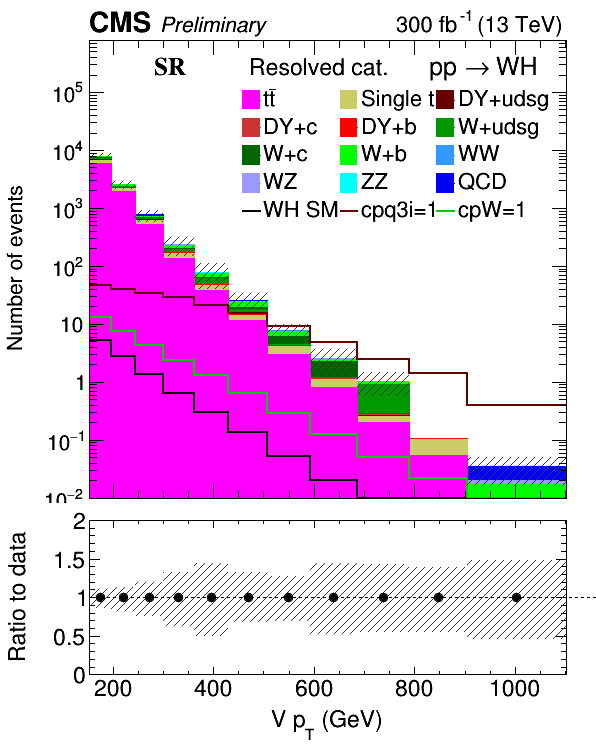
\includegraphics[width=0.475\textwidth]{Figures/RECO/Plot_Resolved_SR_V_pt.png}
%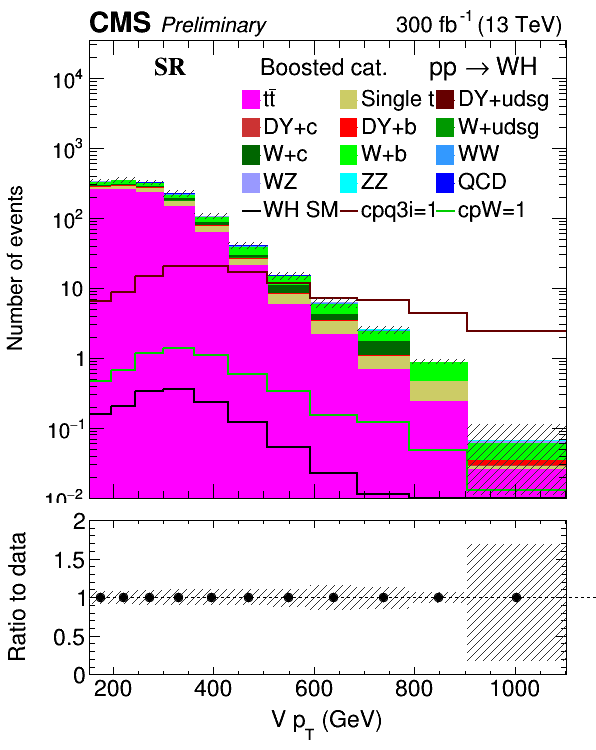
\includegraphics[width=0.475\textwidth]{Figures/RECO/Plot_Boosted_SR_V_pt.png}
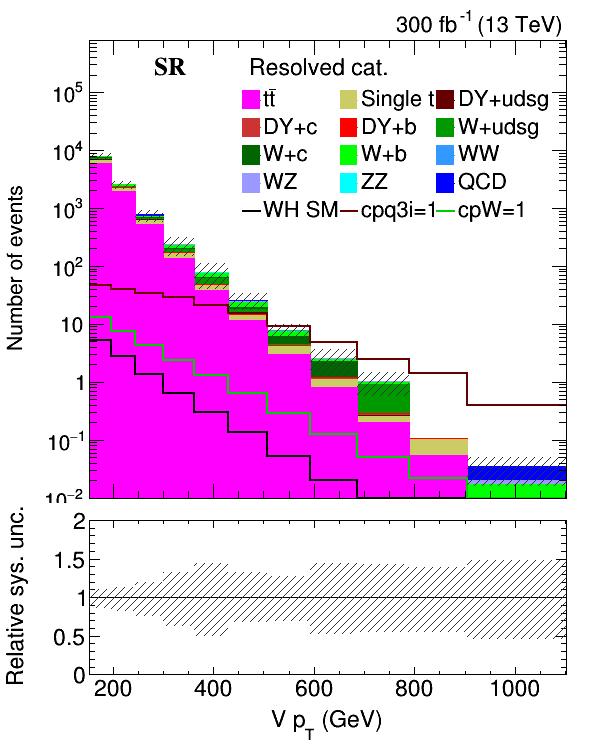
\includegraphics[width=0.475\textwidth]{Figures/New/RECO/Plot_Resolved_SR_V_pt_WH.png}
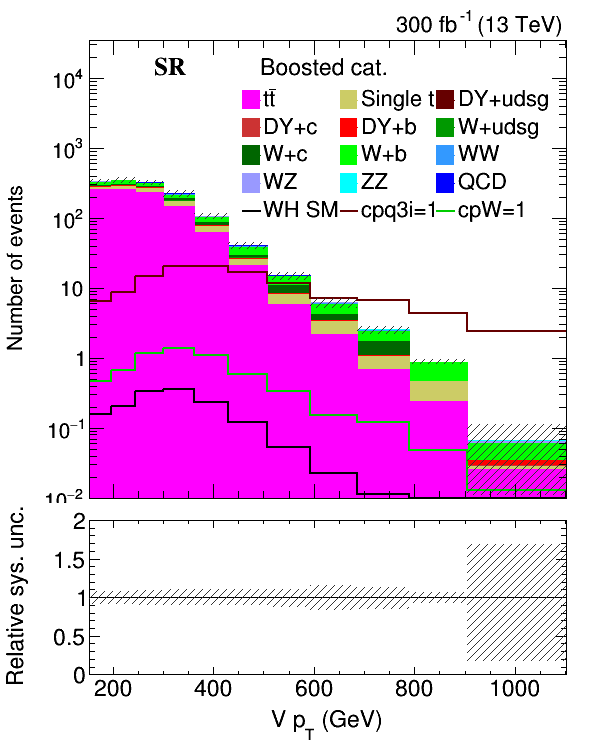
\includegraphics[width=0.475\textwidth]{Figures/New/RECO/Plot_Boosted_SR_V_pt_WH.png}
\end{center}
\caption{
Distribution of \PW boson \pt in the resolved (left) and boosted (left) categories of the SR. Impact of systematic uncertainties on jet energy scale and resolution as well as correction factors used to match the \Pb tagging and Higgs tagging efficiencies in data and simulation are shown in the bottom panel.
}
\label{fig:RECO_Vpt_WH}
\end{figure*}
The figure shows the importance of the $\Pt\PAt$, ${\PW}+\Pb/\Pc$, and ${\PW}+\textrm{udsg}$ backgrounds in the  $\PW\PH$ SRs.
Fig.~\ref{fig:RECO_Vpt_WH} also shows that a large gain in sensitivity to the SM-EFT operators is expected from the high-\pt region, where the signal-to-background ratio improves due to their characteristic energy growth.
%the fact that their contributions grow with energy. 

Next, we turn to the sensitivity of the angular observables after using the selection conditions summarized in Table~\ref{Tab:Regions}. 
%As shown in Fig.~\ref{fig:angles}, 
Distributions of two angular variables $\Theta$ and $\varphi$ in the $\PW\PH$ signal after applying the preselection conditions listed in Table~\ref{Tab:Regions} are shown in Fig.~\ref{fig:angles} for different SM-EFT hypotheses. 
For completeness, similar distributions in the case of the $\PZ\PH$ signal sample are also shown.
Fig.~\ref{fig:angles} shows that
the SM production, dominated by the longitudinal polarization of \PW bosons, exhibits differences in $\Theta$ for nonzero ${\cal O}_{HW}$ coefficients because this operator  enhances the helicity amplitude of $\PW\PH$ production with transversely polarized {\PW} bosons. %FIXME Please check the correctness. --> Done
The observable $\varphi$, on the other hand, is very sensitive to the CP-nature of the \PH--\PV coupling, and the difference in the modulation of CP-even and CP-odd operator coefficients is clearly visible.  
The CP-sensitivity in the $\varphi$ observable is slightly affected by the ambiguities introduced by the unknown $z$-component of the neutrino momentum. %entering the $\PW$ momentum reconstruction. 
This necessitates the development of an algorithm for the neutrino reconstruction, possibly similar to the MVA-based techniques designed in top quark analyses for assigning reconstructed objects to particles produced in the hard interaction~\cite{CMS:2019esx}.
%FIXME Suggest to motivate a selection MVA for the neutrino momentum as we do in tW reco ... adds an action item --> Done
The $\varphi$ observable is weighted by $\sin2\Theta\sin2\theta$ to lift the cancellation otherwise enforced by the triple angular correlation. 
For the first time, we thus resurrect the interference of the helicity amplitudes in \PH final states at the detector level. 
%Comparing these predictions to the Run 2 and 3 data from the CMS experiment is a central goal of this proposal.

\begin{figure*}[hbtp]
\begin{center}
%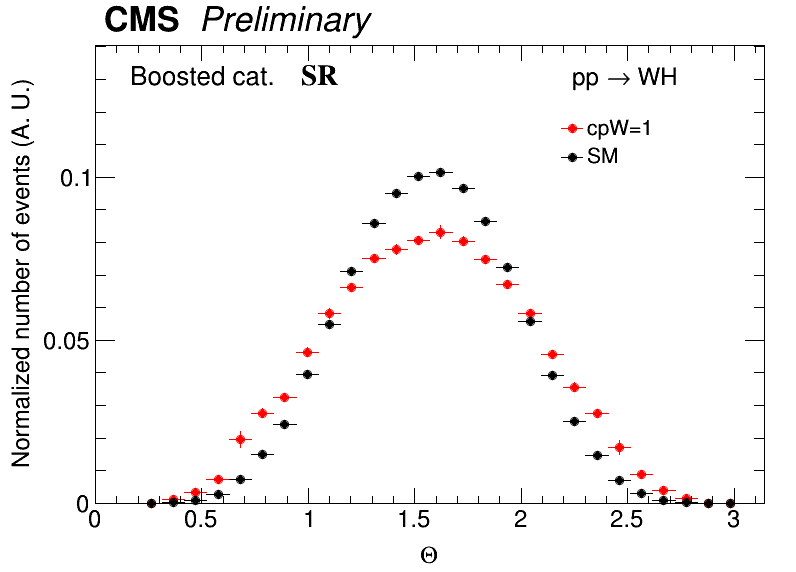
\includegraphics[width=0.475\textwidth]{Figures/RECO/Angle/WH/Boosted_Plot_Theta.png}
%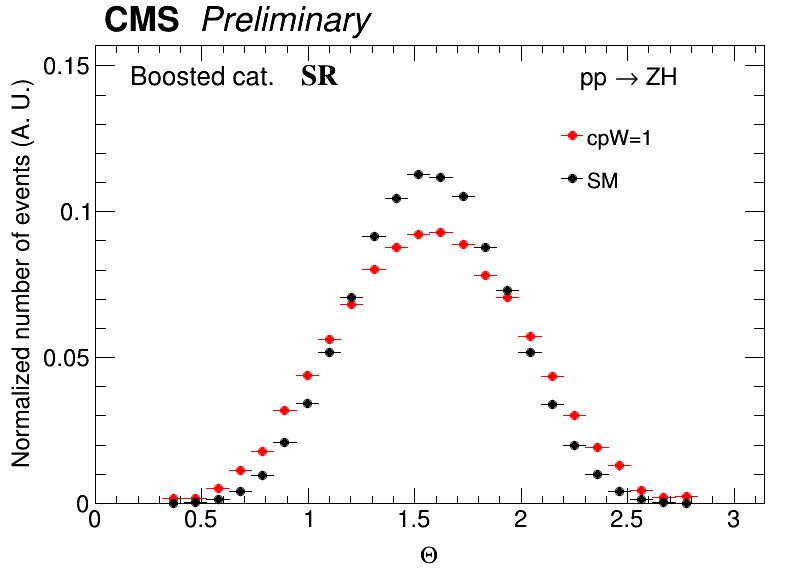
\includegraphics[width=0.475\textwidth]{Figures/RECO/Angle/ZH/Boosted_Plot_Theta.png}
%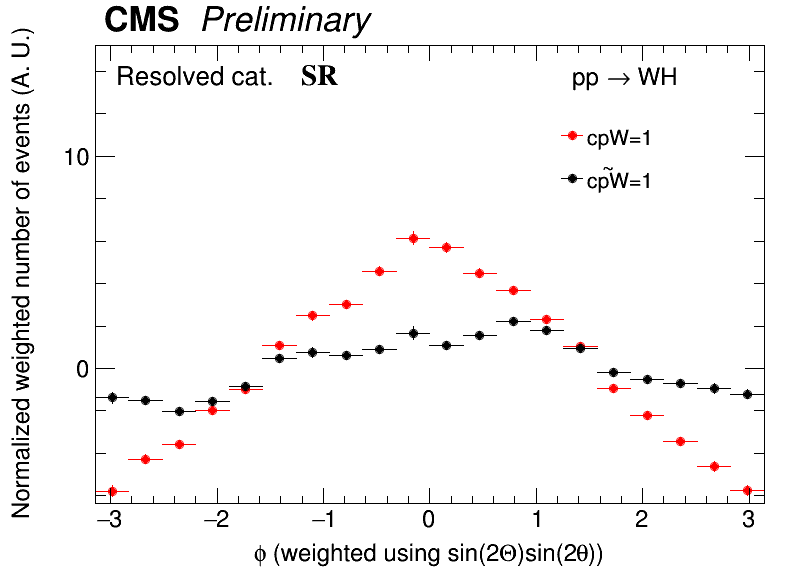
\includegraphics[width=0.475\textwidth]{Figures/RECO/CP/WH/Resolved_Plot_phi.png}
%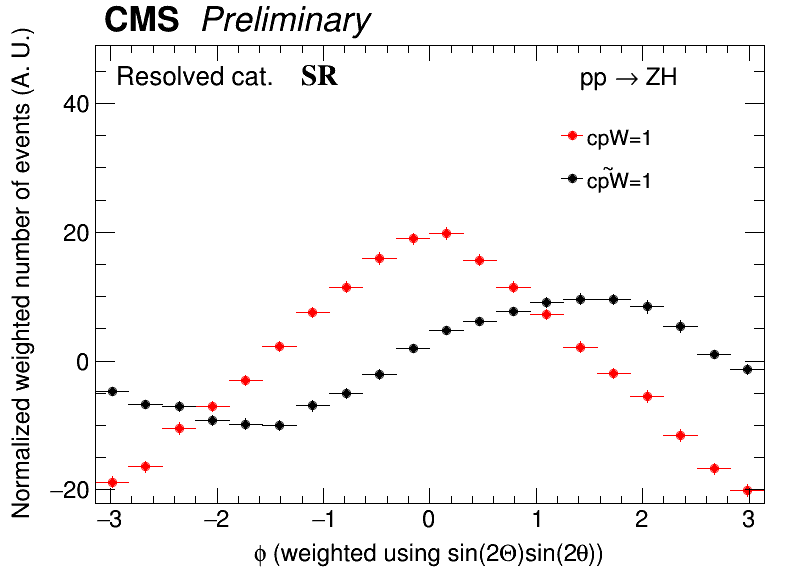
\includegraphics[width=0.475\textwidth]{Figures/RECO/CP/ZH/Resolved_Plot_phi.png}
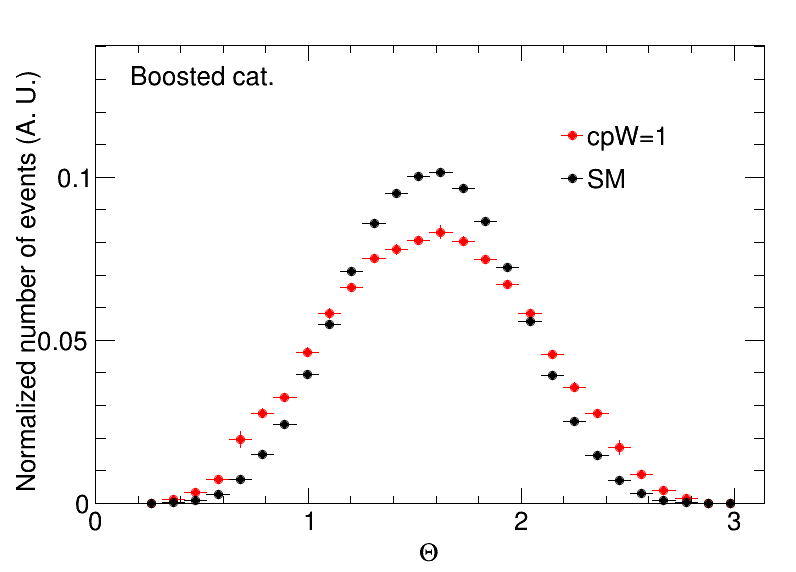
\includegraphics[width=0.475\textwidth]{Figures/New/RECO/Boosted_Plot_Theta_WH.png}
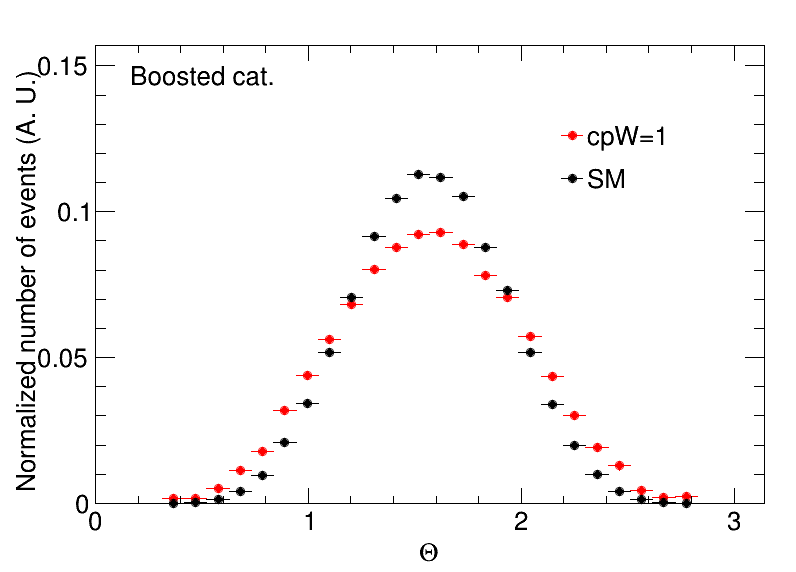
\includegraphics[width=0.475\textwidth]{Figures/New/RECO/Boosted_Plot_Theta_ZH.png}
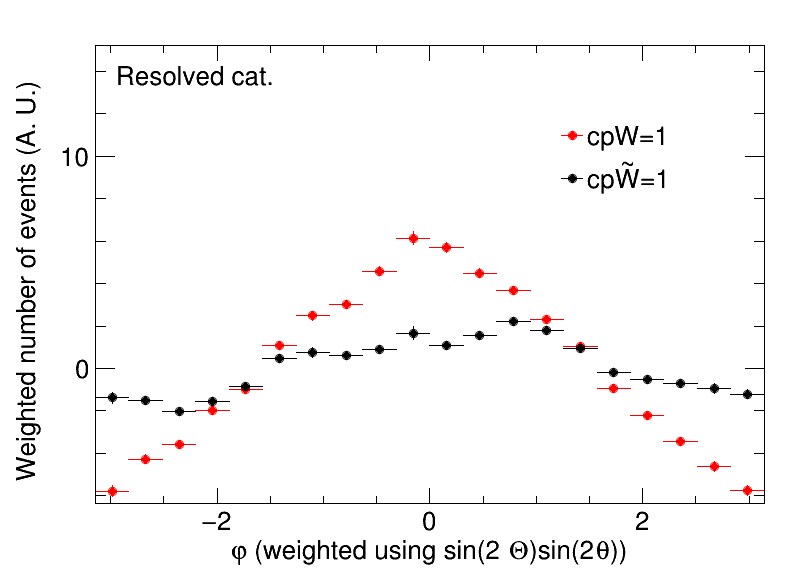
\includegraphics[width=0.475\textwidth]{Figures/New/RECO/Resolved_Plot_phi_WH_CP.png}
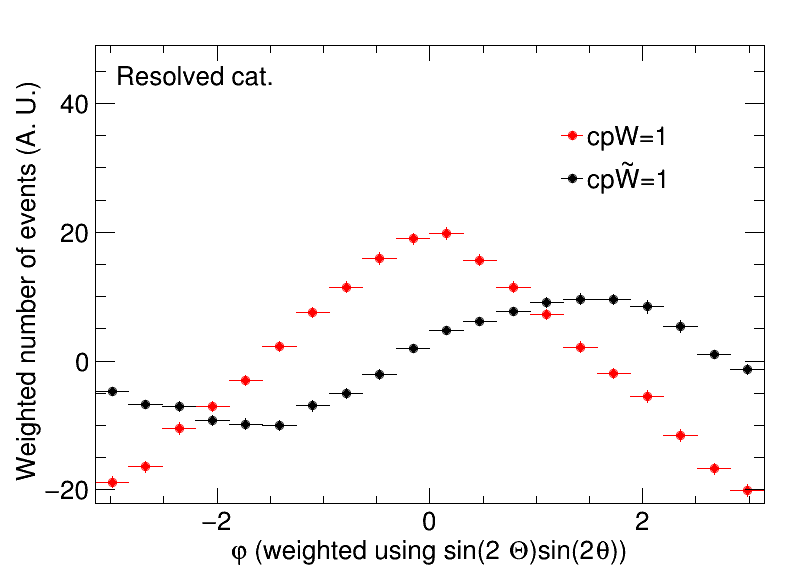
\includegraphics[width=0.475\textwidth]{Figures/New/RECO/Resolved_Plot_phi_ZH_CP.png}
\end{center}
\caption{
Normalized distribution of polar angle $\Theta$ in $\PW\PH$ (top left) and $\PZ\PH$ (top right) signal samples for $cpW=1$ and SM scenarios in the boosted category. 
Normalized distribution of azimuthal angle $\varphi$ in  $\PW\PH$ (bottom left) and $\PZ\PH$ (bottom right) productions for $cpW=1$ and $\tilde{cpW}=1$, respectively; SM component is subtracted from these distributions.
}
\label{fig:angles}
\end{figure*}

\subsection{Neutrino reconstruction}
\label{sec:neu_reco}

In order to reconstruct the momentum of the invisible neutrino in $\PW\rightarrow\Pl\Pgn$, we assume that the \Pnu is the only source of $\ptvecmiss$ in the event and, hence, $\ptvecmiss$ to be equal to the transverse mometum vector of \Pnu. 
In a simple approach, we use the quadratic equation from the $\PW$-mass constraint to calculate $\eta(\Pnu)$. 
The two possible solutions are
\begin{eqnarray}
\eta(\Pnu) &=& {\eta}(l) \pm \cosh^{-1}(1+{\Delta}^2),\;\textrm{where}\label{Eq:NeuEta}\\
{\Delta}^2 &=& \frac{m_W^2 - m_\textrm{T}^2 (\ell,{p_\textrm{T}^\text{miss}\xspace})}{2 p_\textrm{T}^{l}\, p_\textrm{T}^\textrm{miss}}. 
\end{eqnarray}
Large $\pt(\PW)$ leads to $\Delta \ll 1$, and the two solutions become 
\begin{equation}
{\eta}(\Pnu) \simeq {\eta}(\ell) \pm \sqrt{2}{\Delta} + {\cal{O}} ({\Delta}^3)	\ .
\label{Eq:NeuEta2}
\end{equation}
In this limit,  the angular variable $\theta$ and $\Theta$ converge to the same values, whereas a two-fold ambiguity  $\varphi_{+} \simeq \pi - \varphi_{-}$ remains for $\varphi$. 
\begin{figure*}[hbtp]
\begin{center}
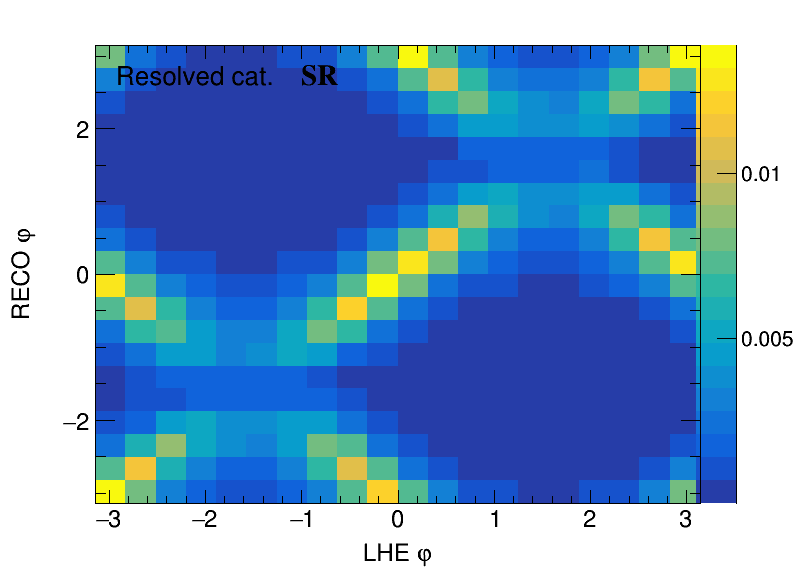
\includegraphics[width=0.495\textwidth]{Figures/New/RECO/Resolved_Plot_2D_phi_unweighted.png}
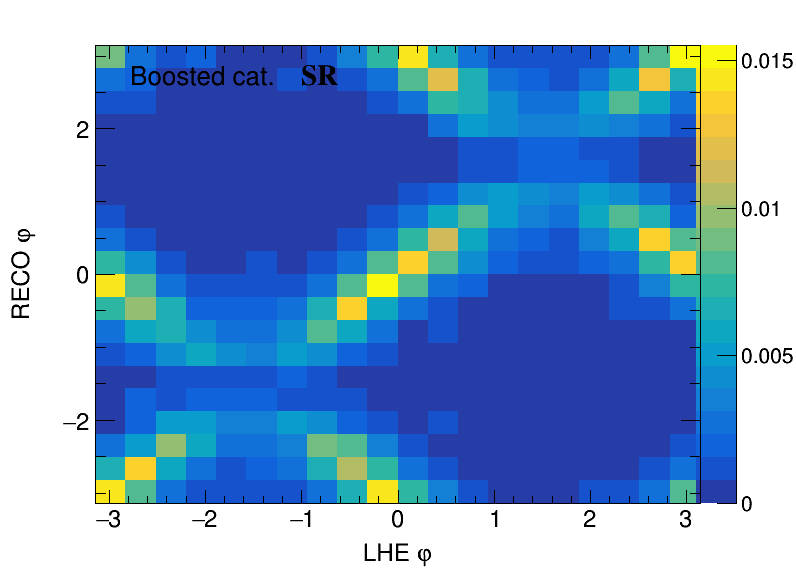
\includegraphics[width=0.495\textwidth]{Figures/New/RECO/Boosted_Plot_2D_phi_unweighted.png}
\end{center}
\caption{
Relation between reconstructed- and parton-level $\varphi$ in the resolved (left) and boosted (right) categories in $\PW\PH$ production illustrating the effect of the ambiguity in the reconstruction of the neutrino momentum. 
}
\label{fig:neureco}
\end{figure*}
This ambiguity is visible in Fig.~\ref{fig:neureco} for the $\PW\PH$ signal sample and currently reduces the CP-sensitivity in $\PW\PH$ production. 
No attempt was made to reduce the impact of the ambiguity for the purpose of this proposal. 
As part of the analysis development, we will develop a multi-variate discriminator to select the correct solution based on the kinematic event properties. %FIXME Add a reference to a successful strategy. --> Added in earlier section

\subsection{Multivariate analysis}

As shown in Fig.~\ref{fig:RECO_Vpt_WH}, the SRs are subject to significant backgrounds from $\Pt\PAt$, ${\PW}+\Pb/\Pc$, and ${\PW}+\textrm{udsg}$. 
%top quark pair  and vector boson production in association with jets.
To separate the  $\PW\PH$ signals optimally from the backgrounds, neural network (NN) discriminators are constructed. 
In this study, it comprises two fully connected dense layers, while the discriminator will be promoted to a DNN 
%in the analysis with real data.
as part of the proposed work.
A very preliminary set of input variables is listed in Table~\ref{Table:MVA_Vars}.
\begin{comment}
Variables in two columns in the upper group are used for the extraction of $\PW\PH$ and $\PZ\PH$ signals, respectively, while
left and right columns in the lower group list variables characterizing the jet system in the resolved and boosted categories, respectively, for the separation of both $\PW\PH$ and $\PZ\PH$ signals from $\Pt\PAt$ background.

{\renewcommand{\arraystretch}{1.3}
\begin{table}[t]
\centering
\caption{
Input variables to the NN discriminator designed to separate events from $\textrm{\PV}\PH$ and $\Pt\PAt$ productions.}
\subcaption*{Lepton-specific variables for $\PW\PH$ (left) and $\PZ\PH$ (right) signals.}
\begin{tabular}{l l}
\pt component of \ptvecmiss &  \pt and $\eta$ of the leading lepton\\
\pt and $\eta$ of the lepton & \pt and $\eta$ of the subleading lepton \\
$\Delta\phi(\Pl,\ptvecmiss)$ & $\Delta\phi({\Pl}_1,{\Pl}_2)$ \\
$\Delta\phi(\PW,\PH)$ & $\Delta\phi(\PZ,\PH)$ \\
Event thrust (see definition in~\cite{CMS:2014tkl}) & Event thrust\\
\end{tabular}
\bigskip
\subcaption*{Variables characterizing the jet system in resolved (left) and boosted (right) categories.}
\begin{tabular}{l l}
B tagging scores of $\textrm{b}_1$ and $\textrm{b}_2$ & DeepAK8 top tagging score \\
$\textrm{Min}(\pt(\textrm{b}_1), \pt(\textrm{b}_2))$ and $\textrm{b}_2$ & DeepAK8 \PW tagging score \\
$\textrm{Max}(\pt(\textrm{b}_1), \pt(\textrm{b}_2))$ & DeepAK8 \PH tagging score \\ 
$\textrm{Max}(\pt(\textrm{b}_1)/\pt(\ell), \pt(\textrm{b}_2)/\pt(\ell))$ & Rapidity and mass of \PH candidate \\
$\Delta\phi(\text{b}_1,\text{b}_2)$ & \\
Rapidity and mass of \PH candidate & \\
AK4 jet multiplicity \\ (satisfying $\pt>30\GeV$, $|\eta|<2.5$)  & \\
\end{tabular}
\label{Table:MVA_Vars}
\end{table}
}
\end{comment}
The variables in the left column of Table~\ref{Table:MVA_Vars} are common to both the resolved and the boosted categories, while the ones in the middle and right columns characterize the jet system in the resolved and the boosted categories, respectively, for the separation of the $\PW\PH$ signal from the $\Pt\PAt$ background.
{\renewcommand{\arraystretch}{1.3}
\begin{table}[t]
\centering
\caption{
Input variables to the NN discriminator designed to separate events from $\textrm{\PV}\PH$ and $\Pt\PAt$ productions.}
\begin{tabular}{l l l}
\pt component of \ptvecmiss & \Pb tagging scores of $\textrm{b}_1$ and $\textrm{b}_2$ & DeepAK8 top tagging score \\
\pt and $\eta$ of the lepton &  $\textrm{Min}(\pt(\textrm{b}_1), \pt(\textrm{b}_2))$ & DeepAK8 \PW tagging score \\
$\Delta\phi(\Pl,\ptvecmiss)$ &  $\textrm{Max}(\pt(\textrm{b}_1), \pt(\textrm{b}_2))$ & DeepAK8 \PH tagging score \\ 
$\Delta\phi(\PW,\PH)$ & $\textrm{Max}(\pt(\textrm{b}_1)/\pt(\ell), \pt(\textrm{b}_2)/\pt(\ell))$ & \\
Rapidity and mass of \PH  &  $\Delta\phi(\text{b}_1,\text{b}_2)$ & \\
Event thrust  & AK4 jet multiplicity  & \\
(see definition in~\cite{CMS:2014tkl}) & (satisfying $\pt>30\GeV$, $|\eta|<2.5$) & \\
\end{tabular}
\label{Table:MVA_Vars}
\end{table}
}
%FIXME Add the following variables to the table. Add also a columns for ZH. --> Done
%A similar discriminator is built in the boosted category using the variables in the left column of Table~\ref{Table:MVA_Vars} along with the following variables corresponding to the \PH candidate AK8 jet: 
%the output of DeepAK8 taggers quantifying the probability of the jet originated due to top quark, Higgs boson, \PW boson relative to the same originated from a light quark or gluon.
Normalized distributions of NN discriminators in SM $\PW\PH$ and $\Pt\PAt$ events are shown in Fig.~\ref{fig:MVA} (left). 
\begin{figure*}[hbtp]
\begin{center}
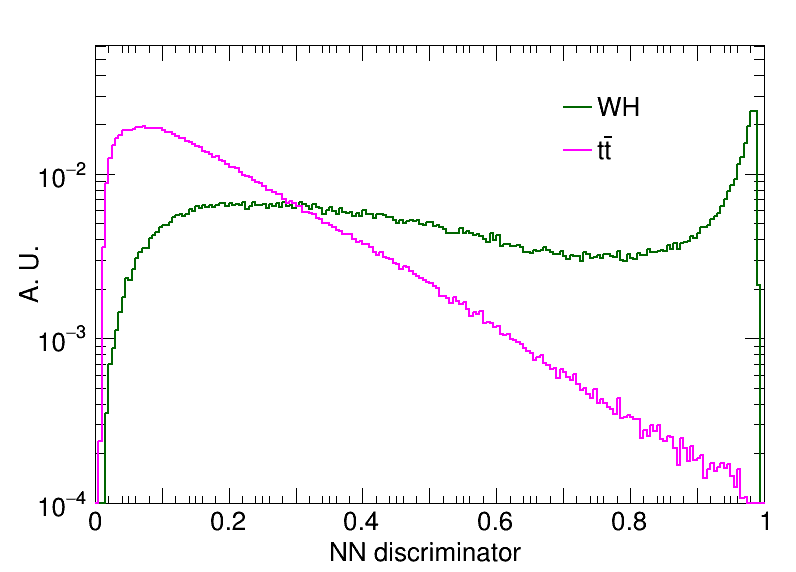
\includegraphics[width=0.3\textwidth]{Figures/New/RECO/Plot_WH_MVA_WH_fast_resolved.png}
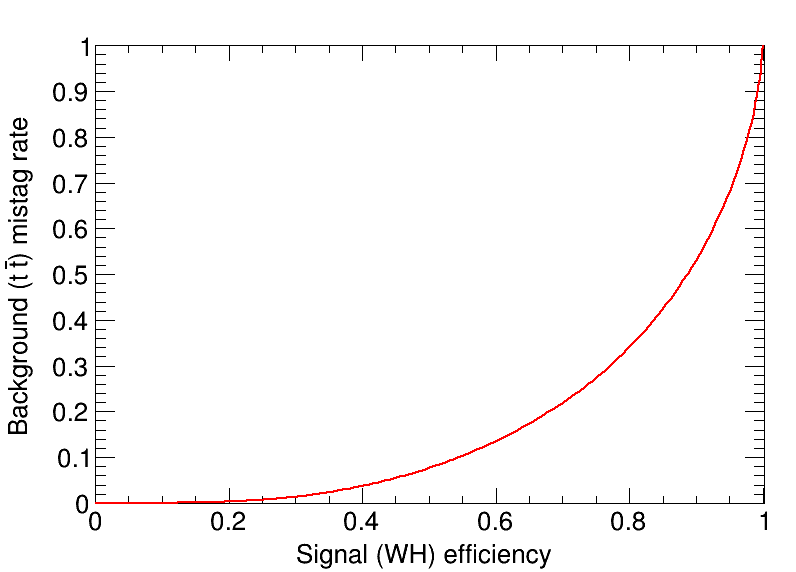
\includegraphics[width=0.3\textwidth]{Figures/New/RECO/ROC_plot_TT_MVA_resolved.png}
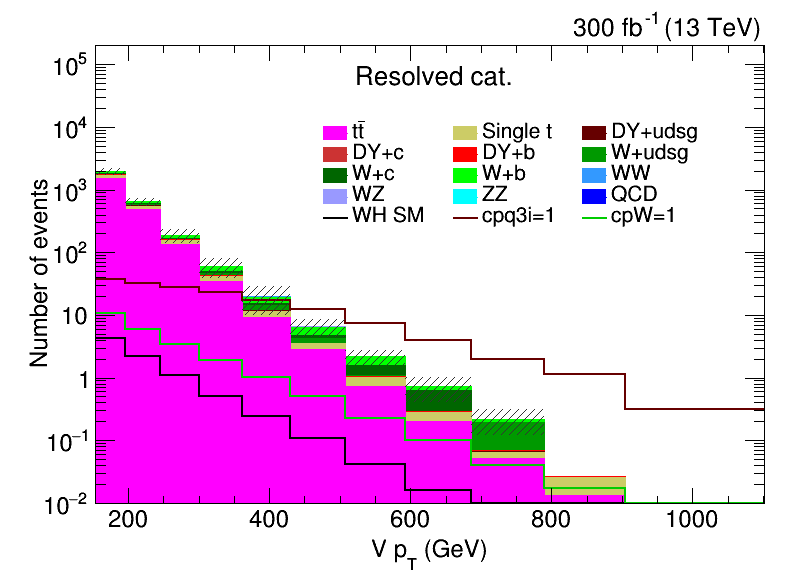
\includegraphics[width=0.3\textwidth]{Figures/New/RECO/Plot_Resolved_SR_V_pt_sigpurity.png}
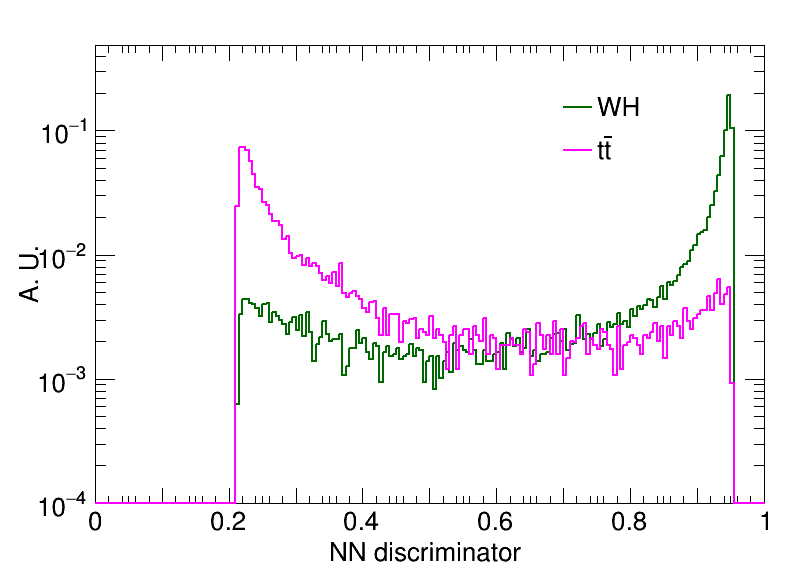
\includegraphics[width=0.3\textwidth]{Figures/New/RECO/Plot_WH_MVA_WH_fast_boosted.png}
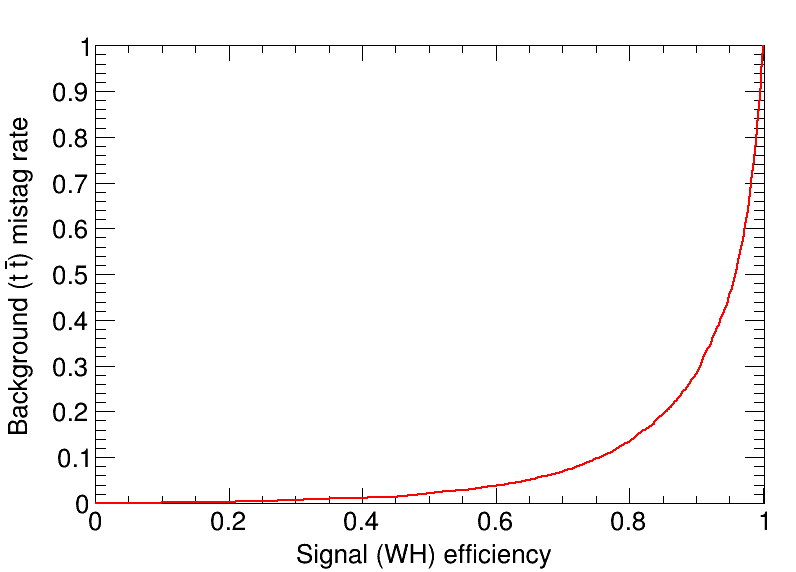
\includegraphics[width=0.3\textwidth]{Figures/New/RECO/ROC_plot_TT_MVA_boosted.png}
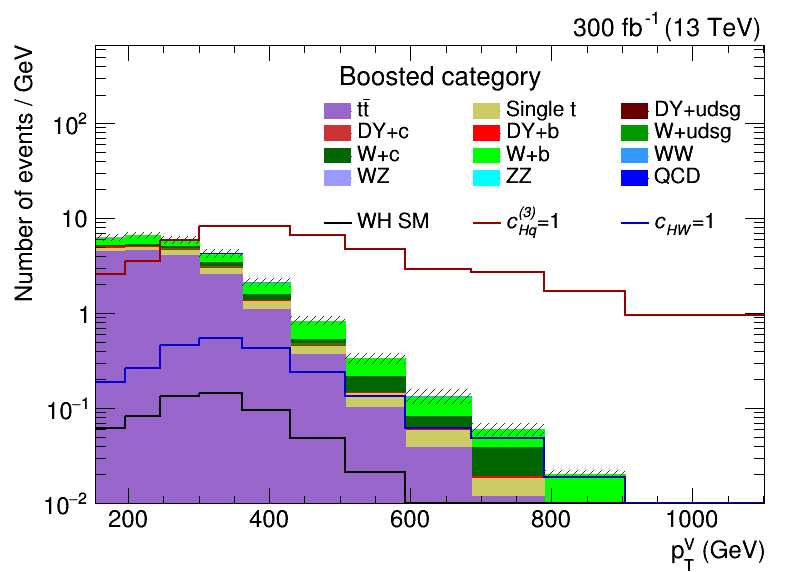
\includegraphics[width=0.3\textwidth]{Figures/New/RECO/Plot_Boosted_SR_V_pt_sigpurity.png}
\end{center}
\caption{
Normalized distributions of the NN discriminator in signal ($\PW\PH$) and background ($\Pt\PAt$) events (left) and ROC curves characterizing the performance of NN discriminator (middle) and  distributions of the \PW boson \pt after applying a condition on the NN discriminator (right) in the resolved (top) and boosted (bottom) categories.
}
\label{fig:MVA}
\end{figure*}
The performance of the discriminator, quantified with resistive operator characteristics (ROC) curves~\cite{FAWCETT2006861}, are shown in Fig.~\ref{fig:MVA} (middle). 
%Benefiting from the DeepAK8 tagger outputs, 
Benefiting from the less combinatorial background,
the discriminator constructed in the boosted category performs slightly better. 
In both cases, the signal distribution is sharply peaked at high discriminator values and no overtraining is observed, indicating a successfully trained classifier.
In the next section, we quantify the sensitivity gain from this strategy.
In the final work, a machine learning based algorithm developed by the applicant's group to separate the SM-EFT effects from the SM~\cite{Chatterjee:2021nms} will be used.

\subsection{Sensitivity results}

Although the final condition on the NN discriminator is subject to development during the project, 
we can obtain a simple assessment of the sensitivity with a threshold on the NN discriminator corresponding to a $\PW\PH$ signal efficiency of $80\%$.
This choice corresponds to a $\Pt\PAt$ background efficiency of $\sim 30\%$ ($\sim 15\%$) in the resolved (boosted) category.
Distributions of the $\PW$ boson \pt after applying this threshold on the NN discriminator are shown in Fig.~\ref{fig:MVA} (right). 
Next, we perform one-dimensional likelihood scans for the Wilson coefficients corresponding to three operators ${\cal O}^{(3)}_{Hq}$, ${\cal O}_{HW}$, and ${\cal O}_{H\tilde{W}}$, respectively, while setting all other Wilson coefficients to $0$. 
In the proposed work, sensitivity for a particular Wilson coefficient will also be measured by allowing others to vary.
Normalizing the predicted yields to an integrated luminosity of 300\fbinv, we show the negative log-likelihood results in Fig.~\ref{fig:NLL}. %FIXME Define q, is it profiled? --> Done
For completeness, the results for the $\PZ\PH$ signal, obtained by following a similar analysis strategy as mentioned for the $\PW\PH$ process, are also combined. 
\begin{figure*}[hbtp]
\begin{center}
%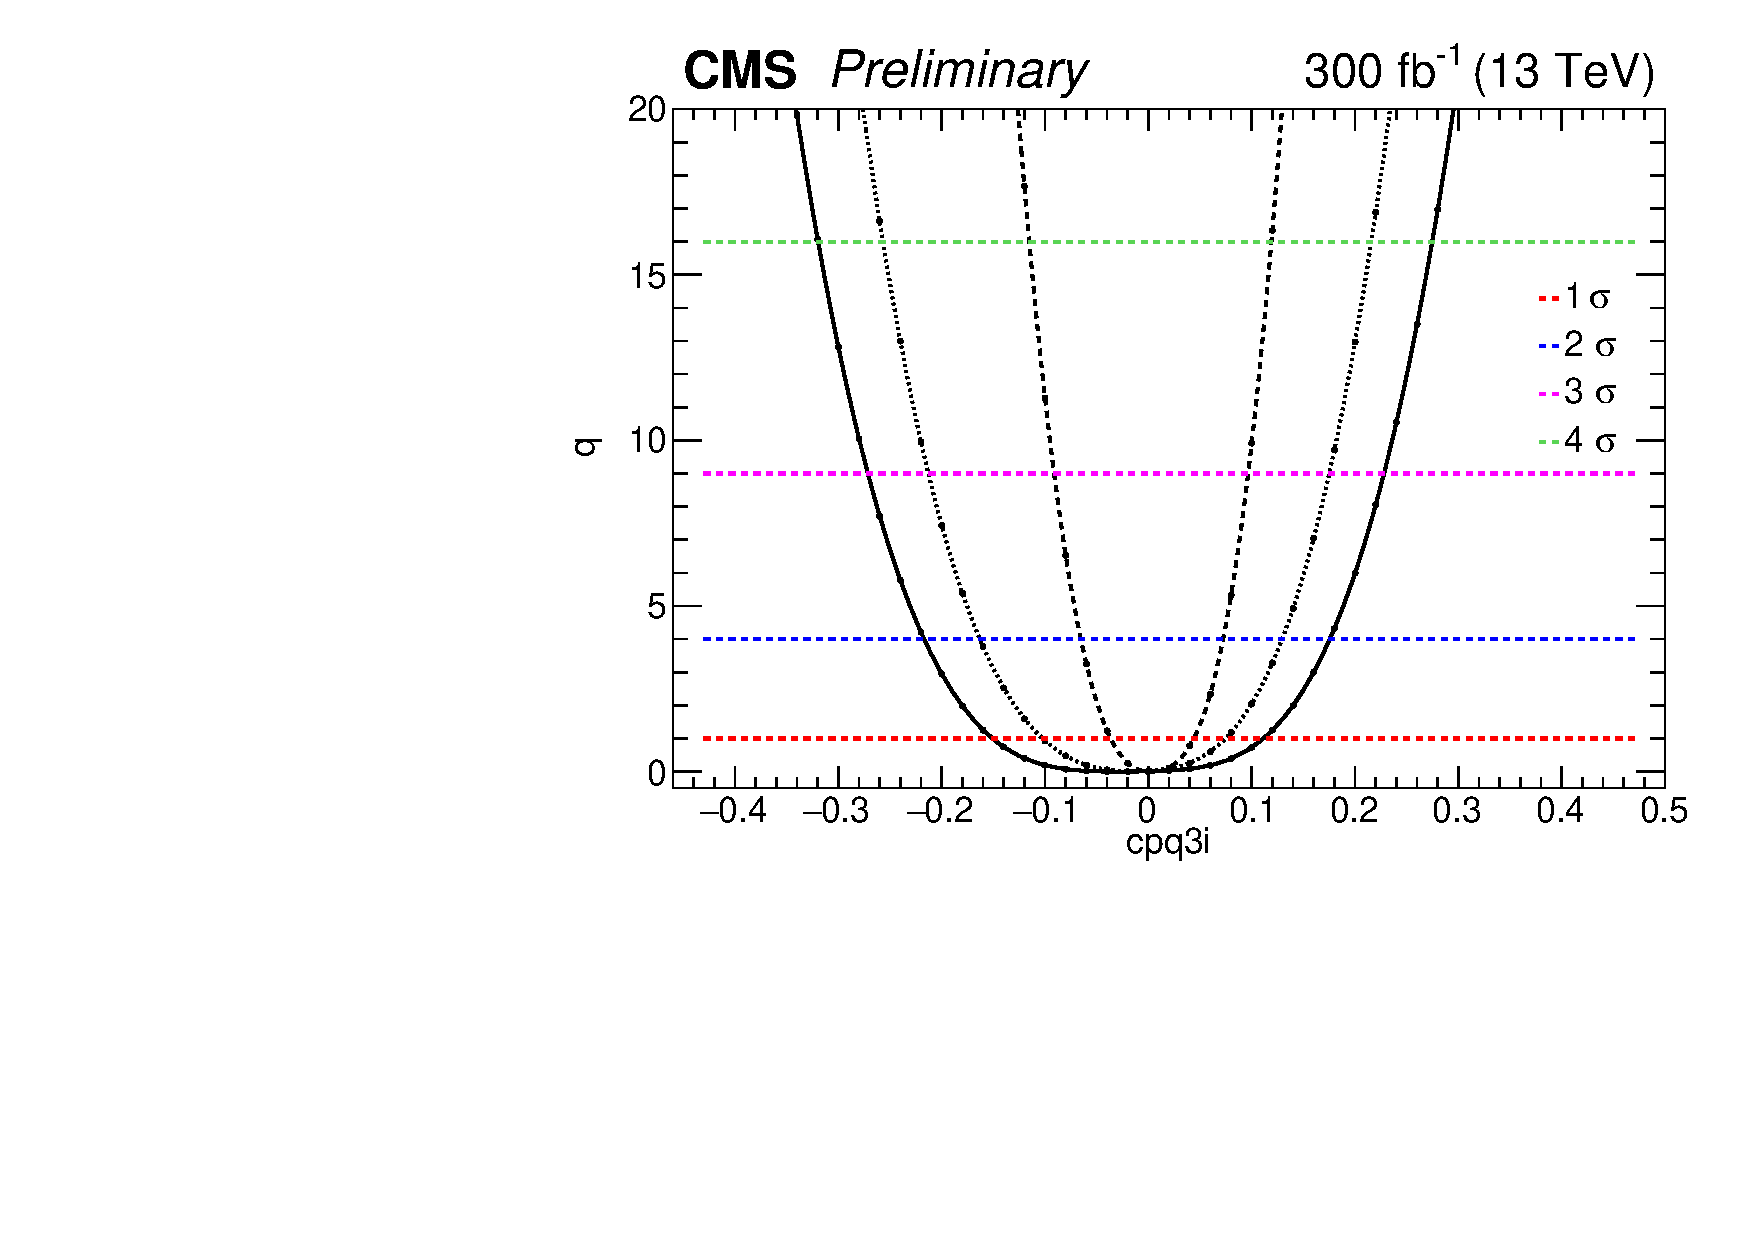
\includegraphics[width=0.495\textwidth]{Figures/RECO/Full_NLL_WC_cpq3i_fine_2019_opt2.pdf}
%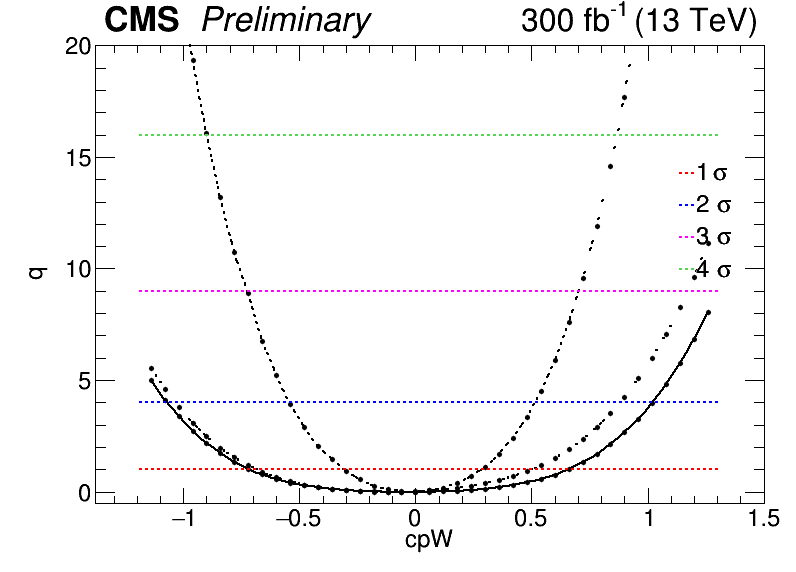
\includegraphics[width=0.495\textwidth]{Figures/RECO/Full_NLL_WC_cpW_fine_2019_opt2.png}
%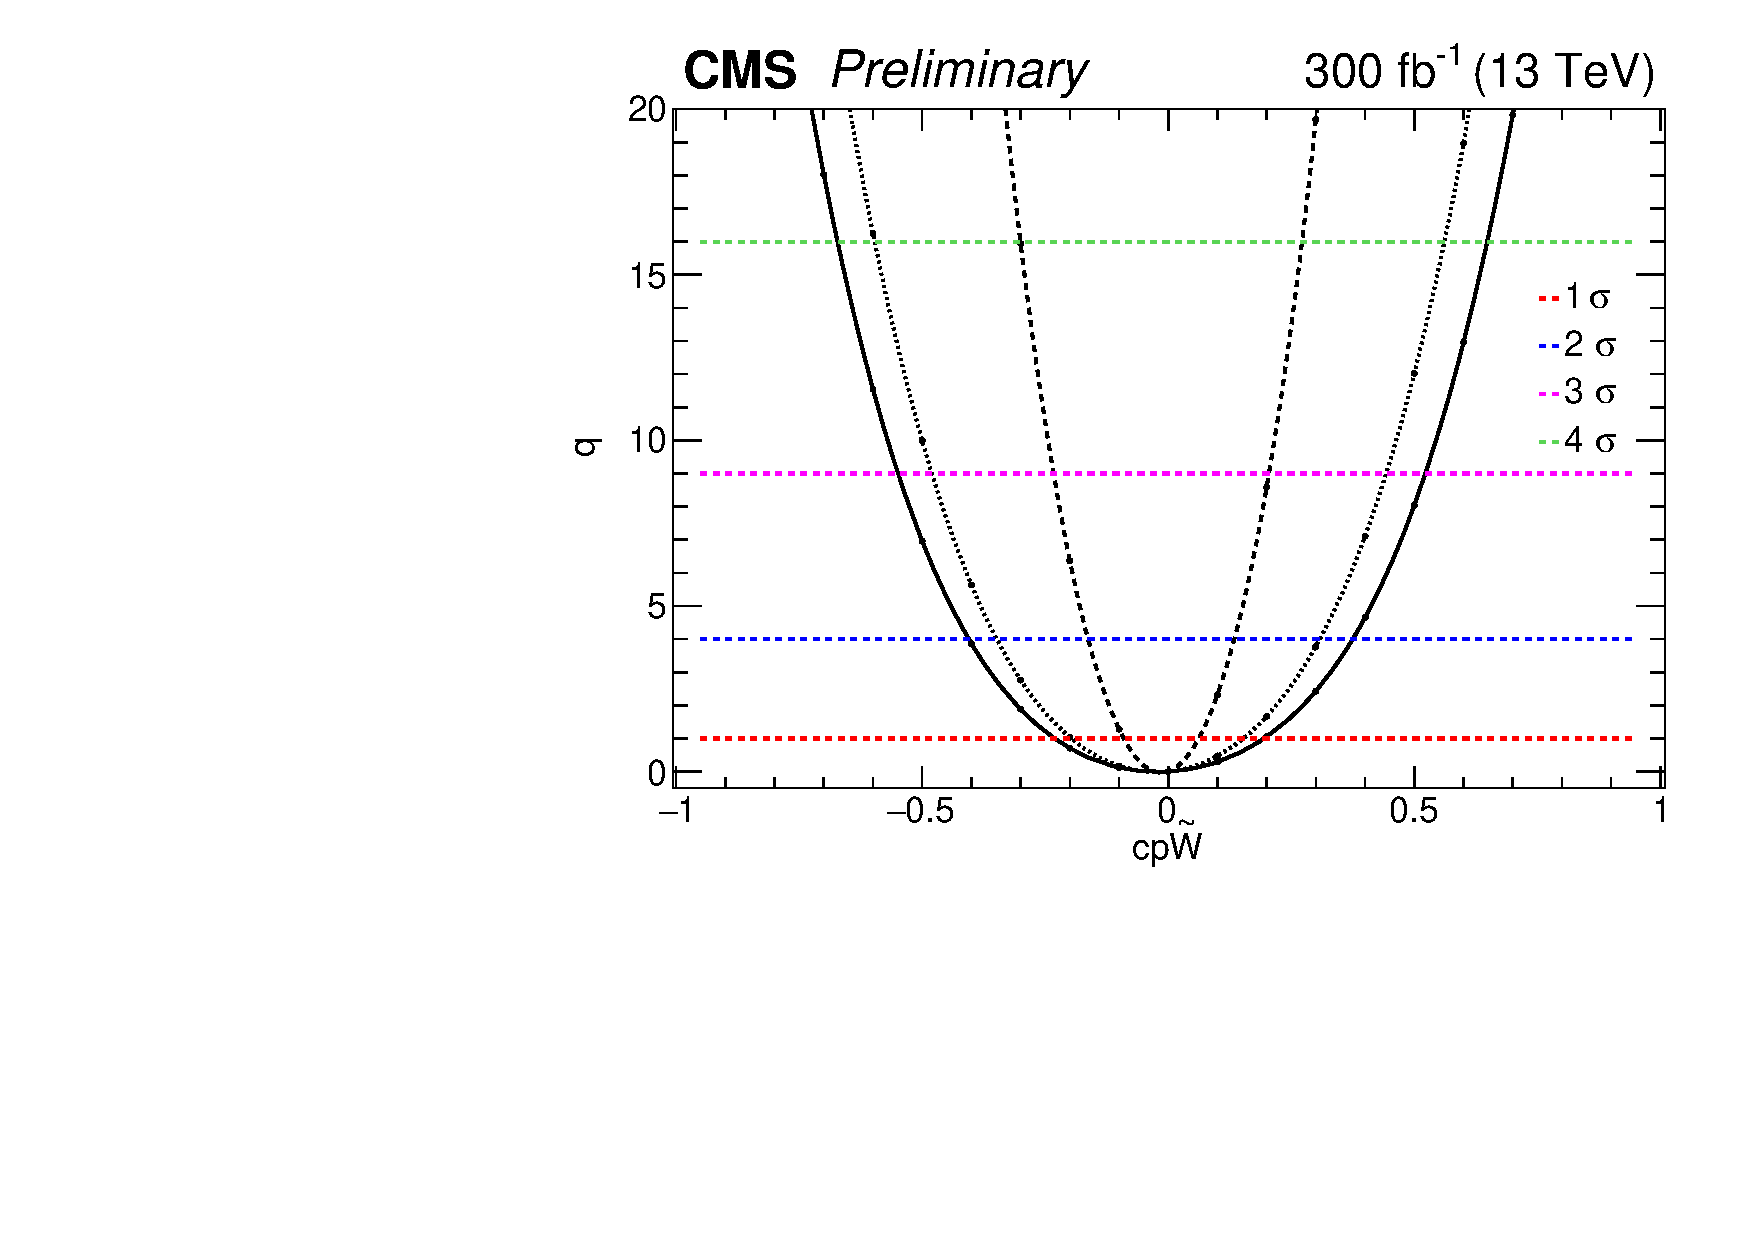
\includegraphics[width=0.495\textwidth]{Figures/RECO/Full_NLL_WC_cpWtilde_2019_opt2.pdf}  
%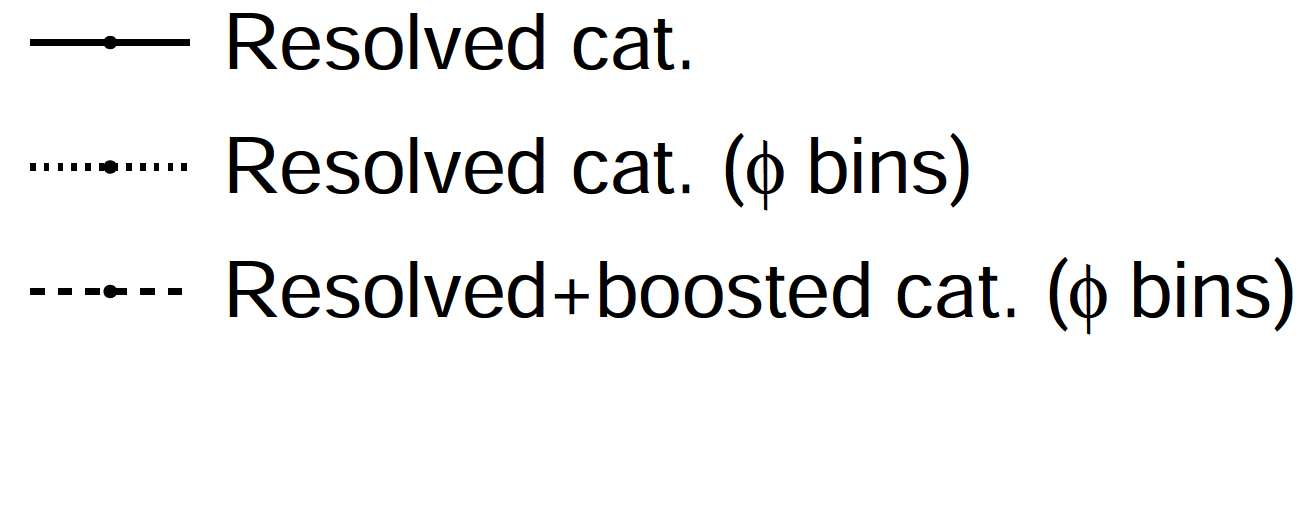
\includegraphics[width=0.495\textwidth]{Figures/RECO/Selection_270.png}
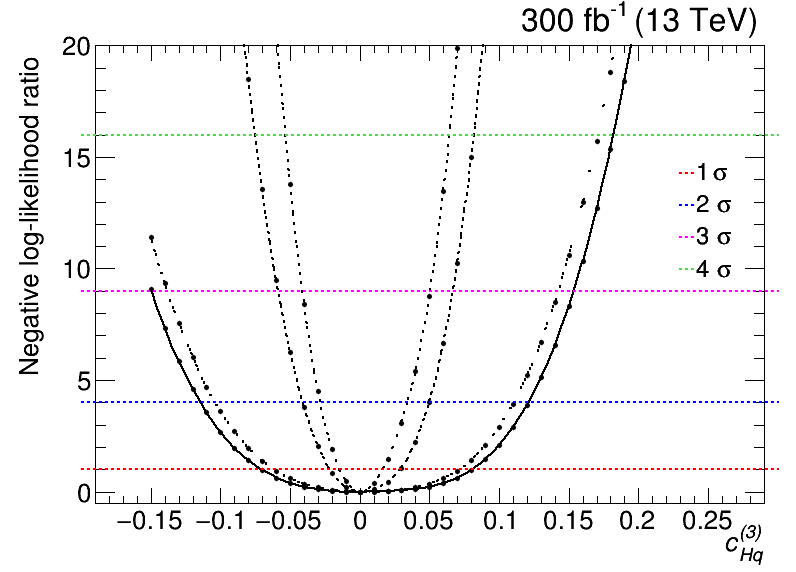
\includegraphics[width=0.49\textwidth]{Figures/New/RECO/Full_NLL_WC_cpq3i_2019_opt2.png}
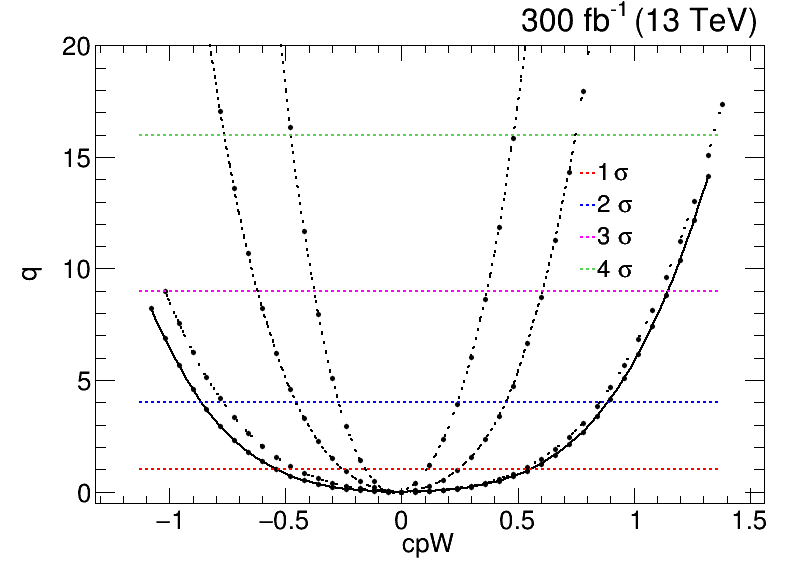
\includegraphics[width=0.49\textwidth]{Figures/New/RECO/Full_NLL_WC_cpW_2019_opt2.png}
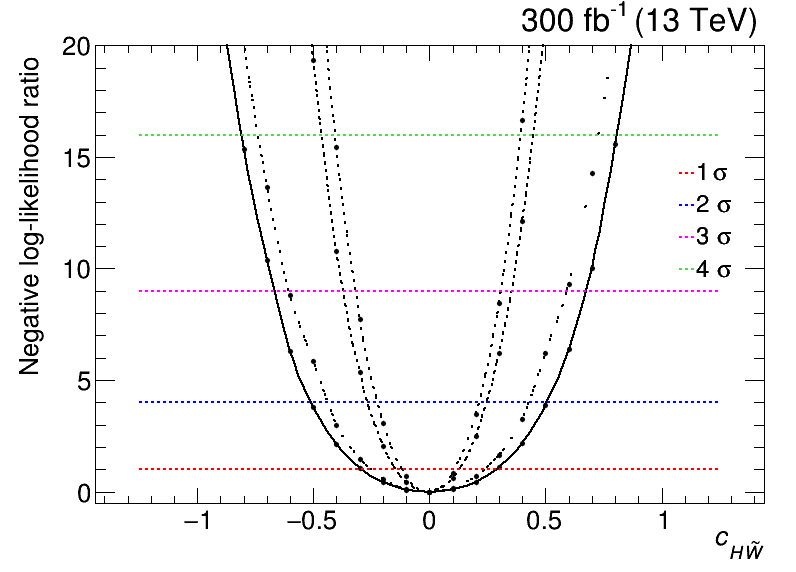
\includegraphics[width=0.49\textwidth]{Figures/New/RECO/Full_NLL_WC_cpWtilde_2019_opt2.png}
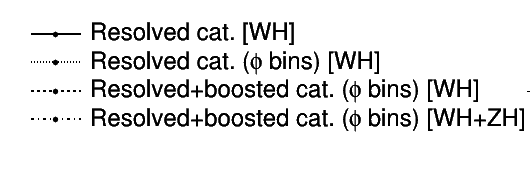
\includegraphics[width=0.495\textwidth]{Figures/New/RECO/Selection_276.png}
\end{center}
\caption{
The profiled likelihood ratio test statistic $q$
%$q = -2\log\frac{L(\vec{\alpha},\vec{\theta})}{L(\hat{\vec{\alpha}},\hat{\vec{\theta})}}$, where $\vec{\alpha}$ and $\vec{\theta}$ denote parameters of interest (POIs) and nuisance parameters, respectively, 
as a function of the Wilson coefficient ${\cal O}^{(3)}_{Hq}$ (top left), ${\cal O}_{HW}$ (top right), and ${\cal O}_{H\tilde{W}}$ (bottom left) for an integrated luminosity of 300\fbinv.
}
\label{fig:NLL}
\end{figure*}
Fig.~\ref{fig:NLL} shows that a large gain in sensitivity is obtained by adding the boosted category due to the energy growth induced by the operators:
%FIXME: We're not yet saying in the beginning that we solve energy growth with the boosted category!! --> Done (added one sentence in research hypothesis and objectives)
The coefficient corresponding to ${\cal O}^{(3)}_{Hq}$ can be constrained to percent level and the ones corresponding to ${\cal O}_{HW}$ and ${\cal O}_{H\tilde{W}}$ within tens of percent at 95\% confidence level with luminosity amounting to 300\fbinv. 
\begin{comment}
Quantitative bounds are presented in Table~\ref{Tab:Limits} at 68\% confidence level.
{\renewcommand{\arraystretch}{1.3}
\begin{table}[htbp]
\caption{Expected bounds at 68\% confidence level on Wilson coefficients corresponding to three operators involved in $\PW\PH$ production for integrated luminosity of 300\fbinv.}
\begin{tabular}{lcl lcl lcl lcl}
\multirow{2}{*}{Operator} &
     \multicolumn{3}{c}{Analysis category} \\
    & Resolved & Resolved w/ $\varphi$ bins & Resolved+boosted w/ $\varphi$ bins \\
    ${\cal O}^{(3)}_{Hq}$    & $\left[-0.16,+0.11\right]$   & $\left[-0.1,+0.08\right]$  & $\left[-0.05,+0.04\right]$ \\
	${\cal O}_{HW}$          & $\left[-0.80,+0.62\right]$   & $\left[-0.78,+0.46\right]$  & $\left[-0.38,+0.26\right]$ \\
	${\cal O}_{H\tilde{W}}$  & $\left[-0.24,+0.22\right]$  &  $\left[-0.22,+0.16\right]$  & $\left[-0.08,+0.06\right]$ \\
  \end{tabular}
\label{Tab:Limits}
\end{table}}
\end{comment}
% Without the boosted category ... %FIXME <- Quantify the gain! --> Done
An improvement due to a binning in $\varphi$ is achieved in the resolved category. 
Addition of the results for the $\PZ\PH$ process improves the sensitivity, particularly for the ${\cal O}_{HW}$ operator coefficient.
The results of this preliminary study are at a similar level as the recent results from the ATLAS Collaboration~\cite{ATLAS-CONF-2021-051},
however, many improvements are expected in the proposed work during its execution.
Also, simultaneous use of information about all three angles $\Theta$, $\theta$, $\varphi$ is expected to result in a significant increase in sensitivity.
The proposed work is also capable of disentangling the effects of CP-even and -odd SM-EFT operators, which is missing in Ref.~\cite{ATLAS-CONF-2021-051}. 
%FIXME Let us discuss this statement in person. Is phi weighted with sinxsin? 

\subsection{P
ossible extensions}

The proposal centers around SM-EFT operators in \VH production, where the gauge boson \PV decays to leptons. 
The methodology developed is also suitable for hadronically decaying \PV; 
the only limitation in the case of $\textrm{\PV}={\PW}$ in sensitivity is the absence of knowledge on \PV charge. 
Latest developments in DNN-based methods for vector boson tagging can be used to increase the sensitivity. 

Strategies developed for the proposed measurement, e.g., background estimation, calibration of trigger efficiencies and \PH tagger, SM-EFT interpretation can also be extended to searches with $\textrm{\PV}\rightarrow \Pl^{+}\Pl^{-} / \Pl \Pgn$ and $\PH \to \Pb \PAb$ in the final state, particularly in the context of a heavy resonance decaying to \PV~and~{\PH}. %FIXME This should be made more concrete. -> Done (maybe partially)

\section{Planned cooperation arrangement} 

The work will be conducted by a PhD student~(N.N.) under the supervision of the principal investigator~(PI) Dr. Suman Chatterjee and within the  CMS data analysis group at the Institute of High Energy Physics (HEPHY) of the Austrian Academy of Sciences. The PI and the PhD student are members of the CMS Collaboration and will work full time on the project. 

The reconstructed data, the simulated background samples, and the object calibration are provided centrally by the CMS Collaboration. 
Ideas and updates will be presented at regular intervals in internal meetings at HEPHY and within the CMS working groups. 
%In general, no cooperative arrangement is planned for this proposal. 

There are synergies with ongoing activities within the HEPHY CMS data analysis group.
The group recently submitted a paper on measuring the $\Pt\PAt\Pgg$ process and constraining the \Pt--\Pgg coupling in SM-EFT; this work was supported by FWF grant P31578.
There is also ongoing work on constraining SM-EFT operators in the $\Pt\PW\PZ$ process supported by FWF grant P33771. 
%Thus the proposed measurement will add a complementary direction in terms of the group's activities.
The existing expertise in the group will help in the smooth execution of the proposed measurement, which will also broaden the scope of the group's activities.

The CMS data analysis group at HEPHY consists of five staff scientists,  three post-doctoral researchers,  and five PhD students working on supersymmetry, long-lived signatures,  searches for BSM Higgs boson decaying to a pair of $\tau$ leptons,  and top quark physics. 
%Diverse experience in the group helps 
The diverse expertise of the group members will help
to develop new ideas and implement those in the CMS Collaboration.

\section{Work and plan}

The work will be carried out by a PhD student~(N.N.) and the applicant and PI Dr. Suman Chatterjee, both working full time on the project. 
%Since the proposed work is on Higgs physics, which is one of the main centers of activities at LHC, the PhD student will get high visibility within the CMS Collaboration.  
In the folloing, the tasks are described in approximate chronological order and are summarized in Table~\ref{tab:workplan}.%Fig.~\ref{fig:workplan}.
\begin{sidewaystable}[t]
\small
  \begin{tabular}{l|c|c|c|c|c|c|c|c|c|c|c|c|c}
    \multirow{2}{*}{Task / Year} &
      \multicolumn{3}{c|}{2022 ($\int \mathcal{L}dt \sim 30$\fbinv)}  &
      \multicolumn{4}{c|}{2023 ($\int \mathcal{L}dt \sim 120$\fbinv)}  & 
      \multicolumn{3}{c|}{2024 ($\int \mathcal{L}dt \sim 160$\fbinv)} &
      \multicolumn{1}{c|}{2025} \\
    & Apr-Jun & Jul-Sep & Oct-Dec & Jan-Mar & Apr-Jun & Jul-Sep & Oct-Dec & Jan-Mar & Apr-Jun & Jul-Dec & Jan-Mar \\
    \hline
    1. Signal simulation for Run~2 & \textcolor{blue}{\checkmark} &  &  &  &  &  &  &  &  &  &     \\
    2. SM-EFT parameterization & \textcolor{orange}{\checkmark} &  &  &  &  &  &  &  &  &  &     \\
    3. Optimization of lepton selection &  & \checkmark & & & &  &  &  &  &  &     \\
    4. Optimization of \Pb tagging condition &  & \textcolor{blue}{\checkmark} & & & &  &  &  &  &  &     \\
    5. Optimization of \PH tagging condition  &  & \textcolor{blue}{\checkmark}& & & &  &  &  &  &  &     \\
    6. Trigger efficiency measurement &  &  & \textcolor{blue}{\checkmark} & & &  &  &  &  &  &    \\
    7. Neutrino reconstruction  &  & & \textcolor{blue}{\checkmark} & & & &  &  &  &  &     \\
    8. Background estimation &  &  &  & \textcolor{blue}{\checkmark} & & &  &  &  &  &     \\
    9. Multivariate analysis &  &  &  & \textcolor{blue}{\checkmark} & & &  &  &  &  &      \\
    10. SM-EFT to SM separation &  &  & & & \textcolor{orange}{\checkmark} & & &  &  &  &       \\
    11. Exp. systematic uncertainties  &  &  &  &  & \textcolor{blue}{\checkmark} & &  &  &  &  &      \\
    12. Modeling uncertainties &  & &  &  & \textcolor{blue}{\checkmark} & & &  &  &  &       \\
    13. Quantification of sensitivity &  & & & & & \textcolor{blue}{\checkmark} & &  &  &  &      \\
    14. SM-EFT effects in background & &  & & & & \textcolor{blue}{\checkmark} & &  &  &  &     \\
    15. Publication based on Run~2 data &  & & & & &  &  & \textcolor{blue}{\checkmark} &  &  &       \\
    16. Signal simulation for Run~3 &  &  & & & &  & \checkmark & &  &  &      \\
    17. Selections for Run~3 & &  & & & &  & \textcolor{blue}{\checkmark} & &  &  &       \\
    18. Choice of \PH tagger for Run~3 &  & & &  &  &  &  &\checkmark  &  &  &      \\    
    19. Background estimation for Run~3 &  & & &  &  & &  &  & \checkmark &  &      \\
    20. Systematic uncertainties for Run~3 &  & &  &  & &  &  &  &  & \checkmark  &      \\
    21. Combination of Run~2 and~3 results &  & & &  &  &  &  &  &  & \textcolor{blue}{\checkmark}  &      \\
    22. Publication of final results &  & & &  &  &  &  & &  &   & \textcolor{blue}{\checkmark}    \\
  \end{tabular}
  \caption{
Tasks shown using symbol \checkmark will be covered by the PhD student, \textcolor{blue}{\checkmark} by the project applicant and PhD student, \textcolor{orange}{\checkmark} by the project applicant and PhD student in collaboration with other members in HEPHY CMS data analysis group.
}
\label{tab:workplan}
\end{sidewaystable}

\begin{enumerate}[noitemsep,topsep=0pt]
\item {\bf Signal simulation for the Run 2 analysis.} Simulate \VH event samples including the effects of SM-EFT operators both at in production and decay using with, e.g., \texttt{SMEFTsim}~\cite{Brivio:2020onw} at leading order or \texttt{SMEFT@NLO}~\cite{Degrande:2020evl} at next-to-leading order in perturbative QCD. 
Particular care needs to be taken for the matching of the hard process generated using {\MGvATNLO}~\cite{Alwall:2014hca} and the parton shower with PYTHIA8~\cite{Sjostrand:2014zea} 
since the parton shower does not involve higher-dimensional operators. Event reconstruction is done within CMS reconstruction software (CMSSW).

\item {\bf SM-EFT parameterization.} Obtain polynomial parametrization of signal yields for arbitrary selections as a function of the Wilson coefficients. Validate the accuracy of the procedure with dedicated simulation of event samples with non-zero Wilson coefficients.

\item {\bf Optimization of the lepton selection.} Optimize the lepton identification criteria  minimizing the total systematic uncertainty. The optimization is done separately for the resolved and the boosted signal regions, as well as for the analysis of the angular observables.
Assess the systematic uncertainty in the angular observables associated with the lepton identification.

\item {\bf Optimization of \Pb tagging criteria.} 
The CMS Collaboration provides the correction to be applied to simulation to match the efficiency of DNN-based \Pb tagging in data and simulation in two variants. 
The first method corrects the simulated efficiency of pre-defined  \Pb tagging working points. 
The second approach is based on reweighting the simulated b-tagging discriminator shape to match the shape observed in data.
Since the \Pb tagging information is used for signal-to-background discrimination, in this task we study the performance and resulting uncertainties for the two options in terms of better overall sensitivity.

\item {\bf Optimization of \PH tagging criterion and scale-factor measurement.} Optimize the DNN-based \PH tagging criterion for signal-to-background separation. 
Measure correction factors need to be measured in appropriate control samples, e.g. in $\PZ\rightarrow\bar \Pqb\Pqb$ event samples, to match the tagging efficiency in data.

\item {\bf Trigger efficiency measurement.} The efficiencies of lepton-based triggers are measured in both data and simulation. 
Corrections to match the trigger efficiency in simulation and data are derived and applied to the simulation. 
%The same needs to be performed for the backup jet triggers. 

\item {\bf MVA based neutrino momentum reconstruction.}
A finely tuned momentum reconstruction is required to resolve the ambiguities in neutrino momentum reconstruction. Using global event observables and kinematic properties of the reconstructed objects, we develop an MVA algorithm based on neural nets to select the correct solution. This task particularly benefits the CP-sensitivity of the \PH--\PW coupling measurements. 
A powerful prescription developed for neutrino reconstruction 
%will also help similar analyses ongoing in CMS. 
will be a valuable asset beyond the scope of this proposal.

\item {\bf Background estimation.} 
%Scaling simulation to measured yields in side band regions is an important method of estimating backgrounds. The procedure is validated in statistically independent selections defined by inverting appropriate selection requirements. %FIXME This item is a bit vague. Can we write 1-2 sentences on a realstic background prediction? -> DONE
%Corrections accounting for  are derived wherever needed, and the corresponding systematic uncertainties are quantified.   
Contributions of background processes will be primarily estimated from the simulation. Orthogonal regions, enriched in important background processes ($\Pt\PAt$, {\PV}+\Pb/\Pc, {\PV}+udsg) will be constructed by inverting the criteria listed in Table~\ref{Tab:Regions}, where the consistency of the simulated background with data will be checked. 
Corrections accounting for mismodeling, if needed, will be derived and the corresponding systematic uncertainties will be quantified. 
Different techniques for the background estimation, e.g., using the mass sidebands, are be checked. 

\item {\bf Multivariate analysis.} Modeling of the variables used for signal-to-background separation in DNN-based multivariate analysis and their correlations need to be properly checked. 
The architecture of the DNN and the threshold on the NN discriminator need to be optimized. 
The modeling of the NN discriminator for different background processes will be checked, 
and data-to-simulation corrections will be derived if needed. 

\item {\bf SM-EFT to SM separation.} In the feasibility study, the constraints on Wilson coefficients are derived just by using a few kinematic variables.
%separating events in different regions. 
A more sophisticated study with a larger number of observables, taking into account their correlation, needs to be performed. 
This will be a test-bed of a method developed by the proposer's group using decision trees~\cite{Chatterjee:2021nms}. 

\item {\bf Experimental systematic uncertainties.} Systematic uncertainties related to different objects, e.g., leptons and jets, and corrections at event-level need to be applied. 
The systematic uncertainties need to be properly derived for the corrections developed during this particular analysis. 
The correlation between systematic uncertainty sources in different years needs to be appropriately defined. 
It will be carefully checked if some of the systematic uncertainties are unexpectedly constrained. 

\item {\bf Modeling uncertainties.} Systematic uncertainties in prediction from the choice of renormalization and factorization scales,  parton distribution function,  and the parton shower need to be derived. 
%and applied to all the predictions taken from simulation. 
The neutrino reconstruction is also expected to be affected by the modeling uncertainties. 

\item {\bf Sensitivity report.} Results from different years of Run~2 will be combined and
the sensitivity of the analysis will be quantified using likelihood scans, taking into account correlations between the operators. 

\item {\bf SM-EFT effects in the background.} So far, all the discussions regarding the SM-EFT operators are made for \VH production, which is the signal targeted. However, some of the operators in Table~\ref{Tab:Operators} also affect some of the background processes. 
For example, ${\cal O}^{(1)}_{Hq}$, ${\cal O}^{(3)}_{Hq}$ affect the diboson production, which is related to \VH production by Goldstone equivalence theorem~\cite{PhysRevD.10.1145} at high energy. 
These are also expected to affect {\PV}+jets production. 
A significant amount of effort needs to be dedicated to the simulation of SM-EFT effects for the backgrounds, followed by a joint analysis of signal and background to report the final sensitivity to the corresponding Wilson coefficients. 

\item {\bf Publication based on Run~2 data.} A first paper will be written reporting the results based on Run~2 data. This involves a series of reviews within the CMS Collaboration and finally by the journal reviewers. 

\item {\bf Signal simulation for Run~3.} The setup developed for the signal simulation for Run~2 will be used in Run~3. However, options will be kept open to incorporate the developments in the theory community by this period. 

\item {\bf Trigger efficiency measurement and optimization of object selection for Run~3.} The triggers which were operational during Run~2 are expected to be available for Run~3 also, but the pileup condition is likely to change. So, the trigger efficiency and corresponding corrections need to be also derived for Run~3. 
For the same reason, object selection criteria need to be reevaluated for Run~3. 

\item {\bf Choice of \PH tagger for Run~3.} With the fast progress in heavy particle tagging, more powerful taggers are expected to be available during the Run~3 schedule. An evaluation will be performed based on the available taggers, and the best performant one will be used. 

\item {\bf Background estimation for Run~3.} Improvements are expected in the Monte Carlo simulation of different processes in the next few years. Thus, the background estimation strategy to be developed for Run~2 analysis will need a validation for Run~3.

\item {\bf Experimental and modeling systematic uncertainties for Run~3.} Systematic uncertainties due to experimental sources will be added. Modeling uncertainties are expected to be very similar to Run~2.

\item {\bf Combination of Run~2 and~3 results.} Results from the analyses based on Run~2 and Run~3 data samples will be combined. Final sensitivity on Wilson coefficients will be reported using the combined data set. 

\item {\bf Publication of final results.} The final results will be reported in a paper, which will go through the internal review process by the CMS Collaboration and finally be submitted to the journal for publication. 

\end{enumerate}


\section{Ethical, safety-related or regulatory aspects}

The sole aim of the project is to improve the human understanding of nature. 
The topic itself has no ethical, safety-related, or regulatory aspects that need to be considered.

\section{Sex-specific and gender-related issues}\label{sec:sex}
The project aims to advance our fundamental understanding of nature. 
Thus the topic itself has no gender-relevant aspects. 
However, the PI is aware of the gender and diversity issues in sciences in general and actively engages in creating equal opportunities for all groups. 
The hiring process at HEPHY is accompanied by a gender-and-diversity officer (Barbara Weber), employed by the institute, who ensures equal opportunities in all communications with candidates. 
W. Adam from HEPHY is a member of the CMS committee for diversity and inclusion and will oversee the hiring process. 
The job advertisement will be formulated gender neutrally. 
In order to improve the gender balance at HEPHY
($23\%$), a suitable female candidate will be given preference.

\section{Human resources}

A PhD student will be recruited solely for this project to be conducted at HEPHY, Vienna. 
The PhD student will carry out the project under the supervision of the project applicant, PI Dr. S. Chatterjee. 
The PI will spend $100\%$ of his time on this project. 
The PI has five years of experience in CMS data analysis in the context of precision jet measurements, searches for new physics, detector calibration, and implementation of algorithms in the CMS software framework. 
The PI has also worked on high energy physics phenomenology in collaboration with theorists and published papers in international journals. 

The tasks will be carried out in consultation with the leader of CMS data analysis group of the institute: Dr. Robert Sch{\"o}fbeck (RS), who is also performing SM-EFT measurements in top quark physics in association with a post-doctoral researcher Dr. Dennis Schwartz (DS). 
Particularly, SM-EFT parameterization (task 2) and SM-EFT to SM separation (task 10) will be performed in collaboration with RS and DS, but they do not take responsibility for the tasks in the work and time plan.
RS is also the former convener of the ``top quark mass and properties'' physics analysis group and the ``Jets and MET'' physics object group of the CMS Collaboration. 
His feedback on documentation and presentation of the results will be constructive. %We'll see.

\appendix
\renewcommand{\thesection}{Annex \arabic{section}} 
\addtocontents{toc}{\setlength{\cftsecnumwidth}{11ex}}

\clearpage
\section{References}
\renewcommand{\refname}{}
{
%\bibliographystyle{jhep}
\bibliographystyle{lucas_unsrt}
\bibliography{VHeft}
}

\newpage

\section{Research institution and required funding}

The Institute of High Energy Physics (HEPHY) of the Austrian Academy of Sciences was founded in 1966. 
Its main purpose is the research in high energy physics and to highlight Austria's membership at CERN. 
On the hardware side, HEPHY has made significant contributions to the CMS inner tracker and to the trigger system. 
The CMS data analysis group, led by Dr. R. Sch{\"o}fbeck, consists of 14 members based at offices in the Apostelgasse 23 in Vienna and at CERN. The successful candidate will be based in Vienna. 
This choice will enable a direct collaboration with the other PhD students and two master students doing data analysis in CMS, as well as with the scientist of the New Physics theory group.
Four members are based at CERN. 
Among them is  W.  Adam, the former physics coordinator of the CMS experiment and the leader of the HEPHY team at CERN.

The infrastructure available to the HEPHY CMS analysis group comprises:
\begin{itemize}
\item Office space with personal workstations at Apostelgasse 23.
\item Access to an LHC-Grid (LCG) Tier-2 cluster with 1000 CPU cores and 500 TByte storage. Access to the CLIP computing cluster at the Gregor Mendel Institute of the Austrian Academy of sciences with approx. 10k CPU cores and 50 TB of
storage for analysis work.
\item Video-conferencing equipment for daily communication with other CMS physicists and participation in CMS Collaboration meetings.
\end{itemize}

This project application requests funding for one PhD student for 48
months (EUR 39.780 per year in 2021). 
The PI S. Chatterjee is a post-doctoral researcher at HEPHY.
Upon a positive funding decision by the FWF, a call for the PhD student will be opened, advertised inside and outside Austria, and made equally accessible to physicists regardless of their race, color, creed, national origin, religion, family status, sexual orientation, age, and political beliefs. 
In order to improve the gender balance at HEPHY ($\sim 23\%$), a suitable female candidate will be given preference.

Furthermore, a total of EUR 5.155 per year for travel expenses between Vienna and CERN is requested. 
These costs are justified as follows: 
The PhD student will travel four times a year (approximately every two months) to CERN for, on average, one week.
The purpose of the four trips is the collaboration with the other experimentalists in the CMS HIG group and to present in person to the other members of the CMS Collaboration.
Also, the PhD student will get the opportunity to participate in the detector operation during the data-taking periods. 
If possible, the CERN trips will overlap with a CMS Collaboration week (internal CMS working meeting occurring four
times a year at CERN). 
Furthermore, one trip to the annual Higgs conference is foreseen, where recent developments in experimental and theoretical results on the Higgs boson are presented. 
The cost for this trip is assumed to be the same as for a trip to CERN.
A breakdown of the expected costs of a working trip to CERN is provided in Table~\ref{Tab:Travel_cost}. 
\begin{table}
\caption{Estimation of travel costs for trips to CERN.}
\begin{center}
{\renewcommand{\arraystretch}{1.3}
\begin{tabular}{m{5 cm}| r r| m {4 cm}}
Item & \multicolumn{2}{c}{Cost} & Comment \\
\hline 
Flight VIE-GVA-VIE & EUR & 300 & \\
7 per diem at EUR 28,10 & EUR & 196,70 & \\
7 per noctem at EUR 24,90 & EUR & 174,30 & \\
6 hotel nights at EUR 60 & EUR & 360  & \\
\hline
Total per year & EUR & 5.155 & 5 trips per year \\
\hline
Total & EUR & 20.620 & For 4 years in total
\end{tabular}
}
\end{center}
\label{Tab:Travel_cost}
\end{table}

The institute needs to pay an amount (memorandum of operation) for the PI, which amounts to EUR 10.000 per year, 
this is also requested in the proposal.
An extra $5\%$ of the total that amounts to EUR 219.740 is requested to cover other unexpected costs.  
Total requested funding sums up to EUR 230.720.  
A summary of the total costs of the project is provided in Table~\ref{Tab:Total_cost}.
\begin{table}
\caption{The total amount of requested funding along with divisions for different items.}
\begin{center}
{\renewcommand{\arraystretch}{1.3}
\begin{tabular}{m{6 cm}| r r}
Item & \multicolumn{2}{c}{ Cost } \\
\hline 
PhD student's salary & EUR & 159.120  \\
PhD student's travel costs of & EUR & 20.620 \\
MoE of the PI (for 3 years) & EUR & 40.000 \\
\hline
General costs ($5\%$) & EUR & 10.980  \\
\hline
Total & EUR & 230.720 
\end{tabular}
}
\end{center}
\label{Tab:Total_cost}
\end{table}

\newpage


\section{CV of the PI}

\subsection*{\underline{Personal Data}}

\textbf{Age:} 27 years (as of February 1, 2021)\\
\textbf{Nationality:} Indian \\
\textbf{Sex:} Male \\
\textbf{Affiliation:} Institute of High Energy Physics of the Austrian Academy of Sciences, 1050 Vienna \\
\textbf{Designation:} Post-doctoral researcher 

%\textbf{PhD Supervisor:} \\ Prof. Gobinda Majumder, \\ Department of High Energy Physics, \\
%Tata Institute of Fundamental Research, Mumbai \\

\subsection*{\underline{Contact Details}}

\textbf{Email:} suman.chatterjee@oeaw.ac.at, suman.chatterjee@cern.ch\\
\textbf{Phone: } +91-7710835260, +43-6769390476\\
\textbf{Personal website: } \href{https://sumanchatterjeetifr.wordpress.com}{https://sumanchatterjeetifr.wordpress.com}


\subsection*{\underline{Academic Records}}

\textbf{2016-2020:}
PhD in Experimental Particle Physics\\
Department of High Energy Physics\\
Tata Institute of Fundamental Research, Mumbai 400005, India\\
\textbf{PhD Supervisor:} Prof. Gobinda Majumder\\
\\
\textbf{2014-2016:}
Master of Science in Physics (Rank: 1st)\\
Tata Institute of Fundamental Research, Mumbai 400005, India\\
\\
\textbf{2011-2014:}
Bachelor of Science in Physics (Remark: 1st class)\\
Department of Physics\\
Jadavpur University, Kolkata  700032, India\\

\subsection*{\underline{Achievements}}

\begin{tabular}{ p{2cm} p{13cm} }
\textbf{2020} & {\textbf{Honorable mention} for the \textbf{IPA Rahul Basu Memorial Award for Best Thesis in High Energy Physics} for the period 2018--2020 in XXIV DAE-BRNS HEP Symposium 2020, India} \\
\textbf{2015} & {\textbf{Professor Sukumar Biswas PhD Student Award for Excellence in Physics} for scoring the highest grades in graduate courses in the Physics Integrated PhD program in Tata Institute of Fundamental Research} \\
%\textbf{2015} \ & Qualified CSIR-UGC National Eligibility Test in Physics with \textbf{All India Rank 43} \\
\textbf{2014} \ & \textbf{All India Rank 3} in Joint Entrance Screening Test 2014 conducted by the research institutes in India  \\
%\textbf{2011-2014} \ &  Awarded \textbf{INSPIRE SCHOLARSHIP} by Department of Science and Technology, India for being within top 1\% students appeared from West Bengal Board of Higher Secondary Education in Higher Secondary (10+2) Examination \\
\textbf{2011} \ & Awarded by the Chief Minister of the state of West Bengal for securing \textbf{the 4$^{\rm{th}}$ rank in the state} in Higher Secondary (10+2) Examination (conducted by West Bengal Council for Higher Secondary Education)  \\
\end{tabular}


\begin{comment}
\subsection*{\underline{CMS Internal Notes \small{(excluding the notes corresponding to the papers)}}}

\textbf{1:} \textit{BSM H$\rightarrow \tau\tau$ analysis on full Run~2 CMS data at $\sqrt{s}=$ 13\,TeV}\\
\ CMS-AN-2020-218\\
\textit{Search for additional Higgs bosons predicted by supersymmetry in the case where the Higgs boson decays into a pair of $\tau$ leptons}\\
\\
\textbf{2:} \textit{Electronic top tagger in CMS}\\
%Suman Chatterjee, Debarati Roy, and Gobinda Majumder \\
\ CMS-AN-2020-168\\
\textit{Implementation and performance monitoring of the algorithm developed in JHEP 01 (2020) 170 in CMS experiment}\\
\\
\textbf{3:} \textit{Implementation of recursive soft drop algorithm in CMS software, and performance studies}\\
%Suman Chatterjee, and Gobinda Majumder \\
\ CMS-AN-2018-070\\
\textit{Implementation of a new jet grooming algorithm, named `recursive soft drop' (JHEP 06 (2018) 093) in CMS software framework and monitoring its performance at HL-LHC}\\
\end{comment}
%\textbf{3:} \textit{Radius scan for inclusive jets in CMS experiment}\\
%Suman Chatterjee, and Gobinda Majumder \\
%\ CMS-AN-2018-044\\

%\textbf{4:} \textit{Upgrade of HO weight factor in particle-flow algorithm}\\
%Suman Chatterjee, and Gobinda Majumder \\
%CMS-DN-2016/023\\


\subsection*{\underline{Oral Presentations at Conferences, Workshops}}

\textbf{September 2021} \ \textbf{Joint annual meeting of Austrian and Swiss physical societies, Innsbruck, Austria} \\
\textit{Parallel talk}\hspace{0.5cm}
SM-EFT results in Higgs sector from the CMS experiment\\
\\
\textbf{July 2021} \ \textbf{European Conference on High Energy Physics 2021, Hamburg, Germany (online)} \\
\textit{Parallel talk}\hspace{0.5cm}
Jet substructure measurements in CMS\\
\\
\textbf{Dec 2020} \ \textbf{XXIV DAE-BRNS HIGH ENERGY PHYSICS SYMPOSIUM 2020} \\
\textit{Rahul Basu Memorial Thesis Award Seminar}\hspace{0.5cm}
Jets as probes for precision measurement and candles for physics beyond standard model\\
\\
\textbf{Jan 2020} \ \textbf{QCD with Electron-Ion Collider, IIT Bombay, Mumbai, India} \\
\textit{Plenary talk}\hspace{0.5cm}
Understanding parton distribution function from LHC measurements\\
\\
\textbf{Sep 2019} \ \textbf{Workshop on Top Quark Physics 2019, IHEP, Beijing, China} \\
\textit{Invited talk}\hspace{0.5cm} 
Heavy resonance searches in ATLAS and CMS \\
\\
\textbf{July 2019} \ \textbf{European Conference on High Energy Physics 2019, Ghent, Belgium} \\
\textit{Parallel talk}\hspace{0.5cm} 
Inclusive jet results from CMS experiment  \\
\\
\textbf{July 2019} \ \textbf{European Conference on High Energy Physics 2019, Ghent, Belgium} \\
\textit{Parallel talk}\hspace{0.5cm}
Tagging top in leptonic decay \\
\\
\textbf{Feb 2019} \ \textbf{International Workshop on Forward and Jet Physics at LHC, Bose Institute, Kolkata, India} \\
\textit{Invited talk}\hspace{0.5cm}
Measurement of inclusive jet cross section and event properties in CMS experiment \\
\\
\textbf{Aug 2018} \ \textbf{QCD at LHC 2018, Technische Universit{\"a}t Dresden, Dresden, Germany} \\
\textit{Parallel talk}\hspace{0.5cm} 
LHC top quark and jet measurements sensitive to PDFs  \\
\\
\textbf{Aug 2018} \ \textbf{QCD at LHC 2018, Technische Universit{\"a}t Dresden, Dresden, Germany} \\
\textit{Parallel talk}\hspace{0.5cm}
Differential jet cross sections at the CMS experiment \\
\\
\textbf{Dec 2017} \ \textbf{WHEPP XV, IISER Bhopal, Bhopal, India} \\
\textit{Parallel talk}\hspace{0.5cm}
Radius Scan for Inclusive Jets in CMS Experiment at $\sqrt{s} =$ 13\,TeV \\
\\
\textbf{Dec 2016} \ \textbf{XXII DAE-BRNS High Energy Physics Symposium, Delhi, India} \\
\textit{Parallel talk}\hspace{0.5cm}
Perspectives for a Radius Scan in Inclusive Jets at 13\,TeV with CMS  \\

\subsection*{\underline{Poster Presentations}}

\textbf{June 2021} \ \textbf{Large Hadron Collider Physics (LHCP 2021) conference, Paris, France (online)}\\
Search for W$^{\prime}$ bosons decaying to a top and a bottom quark at $\sqrt{s}=$ 13\,TeV\\
\\
\textbf{Sep 2018} \ \textbf{Asia-Europe-Pacific School on High Energy Physics, Quy Nohn, Vietnam}\\
Radius scan for inclusive jets at $\sqrt{s}=$ 13\,TeV\\
%\\
%\textbf{Dec 2016} \ \textbf{XXII DAE-BRNS High Energy Physics Symposium, Delhi, India}\\
%HO weight factor in particle flow algorithm in CMS\\

\subsection*{\underline{Teaching Experience}}

\textbf{Autumn 2019: Teaching assistant}\\
Course: Statistical Methods in Physics at TIFR, Mumbai \\
%Instructor: Prof. G. Majumder, TIFR\\
\\
\textbf{January 2019: Co-coordinator}\\
Lecture and hands-on exercise on algorithms used in particle physics for event generation, object reconstruction, and analysis
at the XII School on Experimental High Energy Physics conducted by the Science and Engineering Research Board in India at TIFR, Mumbai \\
\\
\textbf{Autumn 2016: Teaching assistant}\\
Course: Advanced Electrodynamics at TIFR, Mumbai\\
%Instructor: Prof. G. Ravindra Kumar, TIFR\\

\subsection*{\underline{Supervision Experience}}

\textbf{Anirban Bala} (PhD student at TIFR, Mumbai, Advisor: Prof. M. Guchait):\\
During his departmental project I (July-September, 2020) under Prof. G. Majumder \\
Designed the project and mentored thoroughly during its implementation\\

\subsection*{\underline{Organizational Responsibilities}}

\textbf{XII School on Experimental High Energy Physics} at TIFR, Mumbai\\
Helped the organization at the institute level\\
\\
\textbf{SUSY 2017} conference at TIFR, Mumbai\\
Led the team of volunteers \\

\newpage

\section*{{Selected Publications}}

\textbf{1:} {
Search for a W$^\prime$ boson decaying to a top and a bottom quark at $\sqrt{s}=13$\,TeV}\\
CMS Collaboration \\
Phys. Lett. B 820 (2021) 136535 \\
\textit{Most stringent limits published to date on right- and left-handed W$^\prime$ bosons decaying to a top and a bottom quark.}\\
\\
%\textbf{2:} \textit{
%Tree boosting for learning EFT parameters}\\
%arXiv:2107.10859\\
%\textit{A new tree boosting algorithm designed for the measurement of parameters in the context of effective field theory.}
%\\
\textbf{2:} {
Dependence of inclusive jet production on the anti$\mbox{-}k_T$ distance parameter in pp collisions at $\sqrt{s} = 13$\,TeV}\\
CMS Collaboration \\
JHEP 12 (2020) 082\\
\textit{First public results from colliders on dependence of inclusive jet cross section on jet size.}\\
\\
\textbf{3:} {Calibration of the CMS hadron calorimeters using proton-proton collision data at $\sqrt{s}= 13$\,TeV}\\
CMS Collaboration \\
JINST 15 (2020) P05002\\
\textit{Absolute calibration of outer hadron calorimeter in particle-flow algorithm in CMS.}\\
\\
\textbf{4:} {Jets with electrons from boosted top quarks}\\
Suman Chatterjee, Rohini Godbole, and Tuhin S. Roy\\
JHEP 01 (2020) 170\\
\textit{An algorithm to identify boosted top quarks decaying where W boson from top quark decays to an electron using jet substructure techniques.}\\
\\
\textbf{5:} {Mixed WIMP-axion dark matter}\\
Suman Chatterjee, Anirban Das, Tousik Samui, and Manibrata Sen\\
Phys. Rev. D 100, 115050\\
\textit{A detailed study of the phenomenology of a multi-component dark matter scenario with
a scalar WIMP and the QCD axion in the light of the latest data from dark matter detection experiments and
LHC results.}\\
\\
%\textbf{7:} \textit{Les Houches 2017: Physics at TeV Colliders Standard Model Working Group Report}\\
%arXiv:1803.07977 \\
%\textit{A detailed study of two-prong taggers and measurement of strong coupling using jet substructure}
%\\
\textbf{6:} {Dose rate effects in the radiation damage of the plastic scintillators of the CMS hadron endcap calorimeter}\\
CMS Collaboration \\
2016 JINST 11 T10004\\
%arXiv:1608.07267\\
\textit{Measurements of change in light output by plastic scintillators in the CMS hadron endcap due to irradiation during the collisions at LHC at $\sqrt{s} = 8$\,TeV.}\\


%------------------------------------------------

\end{document}
